\documentclass[letterpaper,10pt,headsepline]{scrbook}
\usepackage[T1]{fontenc} 
\usepackage{natbib}
\usepackage{supertabular}
\usepackage{epsfig}
\usepackage{ifthen}
\usepackage{index}
\usepackage{xr-hyper}
\usepackage[backref,colorlinks]{hyperref}
\usepackage{listings}
\usepackage{verbatim}
\usepackage{hyphenat}
\usepackage{ragged2e}
\usepackage[acronym]{glossaries}
\usepackage{color}
\usepackage{tensor}
\usepackage{textcomp}

% Adaptive labelling.
\makeatletter
\newcommand{\iflabelexists}[3]{\@ifundefined{r@#1}{#3}{#2}}
\makeatother

% Names
\def\glc{{\normalfont \scshape Galacticus}}

% Reference main Galacticus documentation.
\externaldocument[main-]{../../galacticus/doc/Galacticus}[https://users.obs.carnegiescience.edu/abenson/galacticus/Galacticus_v0.9.4.pdf]

% Table of contents
\setcounter{tocdepth}{5}

% Margins.
\setlength{\topmargin}{0mm}
\setlength{\textwidth}{160mm}
\setlength{\textheight}{210mm}
\setlength{\oddsidemargin}{0mm}
\setlength{\evensidemargin}{0mm}

\makeglossary
\glstoctrue
\makeindex

% Acronyms.
\newacronym{cmb}{CMB}{cosmic microwave background}
\newacronym{igm}{IGM}{intergalactic medium}
\newacronym{imf}{IMF}{initial mass function}
\newacronym{isco}{ISCO}{innermost stable circular orbit}
\newacronym{ism}{ISM}{interstellar medium}
\newacronym{ode}{ODE}{ordinary differential equation}
\newacronym{nfw}{NFW}{Navarro-Frenk-White (dark matter halo profile)}
\newacronym{sed}{SED}{spectral energy distribution}
\newacronym{sne}{SNe}{supernovae}
\newglossaryentry{adaf}{type=\acronymtype, name={ADAF}, description=\glslink{adafg}{advection-dominated accretion flow}, first={advection-dominated accretion flow (ADAF)}, see=[Glossary:]{adafg}}
\newglossaryentry{pah}{type=\acronymtype, name={PAH}, description=\glslink{pahg}{polycyclic aromatic hydrocarbon}, first={polycyclic aromatic hydrocarbon (PAH)}, see=[Glossary:]{pahg}, firstplural={polycyclic aromatic hydrocarbons (PAH)}, see=[Glossary:]{pahg}}
\newglossaryentry{dsl}{type=\acronymtype, name={DSL}, description=\glslink{dslg}{domain-specific language}, first={domain specific language (DSL)}, see=[Glossary:]{dslg}, firstplural={domain-specific languages (DSLs)}, see=[Glossary:]{dslg}}
\newglossaryentry{wdm}{type=\acronymtype, name={WDM}, description=\glslink{wdmg}{warm dark matter}, first={warm dark matter (WDM)}, see=[Glossary:]{wdmg}, firstplural={warm dark matters (WDM)}, see=[Glossary:]{wdmg}}
\newacronym{sdss}{SDSS}{Sloan Digitial Sky Survey}
\newglossaryentry{ahf}{type=\acronymtype, name={AHF}, description=\glslink{ahfg}{Amiga's Halo Finder}, first={Amiga's Halo Finder (AHF)}, see=[Glossary:]{ahfg}}
\newglossaryentry{cdm}{type=\acronymtype, name={CDM}, description=\glslink{cdmg}{cold dark matter}, first={cold dark matter (CDM)}, see=[Glossary:]{cdmg}, firstplural={cold dark matters (CDM)}, see=[Glossary:]{cdmg}}
\newacronym{mcmc}{MCMC}{Markov Chain Monte Carlo}
\newglossaryentry{sam}{type=\acronymtype, name={SAM}, description=\glslink{samg}{semi-analytic model}, first={semi-analytic model (SAM)}, see=[Glossary:]{samg}, firstplural={semi-analytic models (SAMs)}, see=[Glossary:]{samg}}
\newglossaryentry{bie}{type=\acronymtype, name={BIE}, description=\glslink{bieg}{semi-analytic model}, first={Bayesian inference engine (BIE)}, see=[Glossary:]{bieg}, firstplural={Bayesian inference engines (BIEs)}, see=[Glossary:]{bieg}}
\newglossaryentry{hod}{type=\acronymtype, name={HOD}, description=\glslink{hodg}{halo occupation distribution}, first={halo occupation distribution (HOD)}, see=[Glossary:]{hodg}, firstplural={halo occupation distributions (HODs)}, see=[Glossary:]{hodg}}
\newglossaryentry{mpi}{type=\acronymtype, name={MPI}, description=\glslink{mpig}{message passing interface}, first={message passing interface (MPI)}, see=[Glossary:]{mpig}, firstplural={message passing interfaces (MPIs)}, see=[Glossary:]{mpig}}
\newglossaryentry{hdf5}{type=\acronymtype, name={HDF5}, description=\glslink{hdf5g}{hierarchical data format}, first={hierarchical data format (HDF5)}, see=[Glossary:]{hdf5}, firstplural={hierarchical data formats (HDF5s)}, see=[Glossary:]{hdf5g}}
\newglossaryentry{pbs}{type=\acronymtype, name={PBS}, description=\glslink{pbsg}{portable batch system}, first={portable batch system (PBS)}, see=[Glossary:]{pbsg}, firstplural={portable batch systems (PBSs)}, see=[Glossary:]{pbsg}}
\newglossaryentry{pdf}{type=\acronymtype, name={PDF}, description=\glslink{pdfg}{probability density function}, first={probability density function (PDF)}, see=[Glossary:]{pdfg}, firstplural={probability density functions (PDFs)}, see=[Glossary:]{pdfg}}
\newglossaryentry{cdf}{type=\acronymtype, name={CDF}, description=\glslink{cdfg}{cumulative distribution function}, first={cumulative distribution function (CDF)}, see=[Glossary:]{cdfg}, firstplural={cumulative distribution functions (CDFs)}, see=[Glossary:]{cdfg}}
\newglossaryentry{gsl}{type=\acronymtype, name={GSL}, description=\glslink{gslg}{GNU Scientific Library}, first={GNU Scientific Library (GSL)}, see=[Glossary:]{gslg}}
\newglossaryentry{gama}{type=\acronymtype, name={GAMA}, description=\glslink{gamag}{Galaxy and Mass Assembly}, first={Galaxy and Mass Assembly (GAMA)}, see=[Glossary:]{gamag}}

% Glossary entries.
\newglossaryentry{FFTLog}{name={FFTLog}, description={\href{http://casa.colorado.edu/~ajsh/FFTLog/}{FFTLog} is a code to compute fast Fourier transforms of discrete periodic sequences of logarithmically spaced data}}

\newglossaryentry{component}{name={component}, description={An individual physical system within a \gls{node}, such as a dark matter halo, a galactic disk or a supermassive black hole}}

\newglossaryentry{forest}{name={forest}, description={A collection of merger trees that are linked together by virtue of nodes which jump between trees}}

\newglossaryentry{node}{name={node}, description={A single point in a merger tree, consisting of a dark matter halo and associated baryons}}

\newglossaryentry{mergee}{name={mergee}, description={For a given node in a merger tree, the set of mergee nodes consists of all nodes which will undergo a galaxy merger with the node at some point in the future}}

\newglossaryentry{primary progenitor}{name={primary progenitor}, description={The progenitor of a given \gls{node} which is regarding as the direct descendent of that \gls{node} (often, but not always, the most massive progenitor). Other progenitors are considered to merge into this primary progenitor}}

\newglossaryentry{parent}{name={parent}, description={In a merger tree, the parent node of any given node that exists at time $t_0$ is that node to which it is directly connected in the tree at time $t_1>t_0$}}

\newglossaryentry{Bernoulli distribution}{name={Bernoulli distribution}, description={A discrete probability distribution which takes value $1$ with success probability $p$ and value $0$ with failure probability $q = 1-p$. Read more on \href{http://en.wikipedia.org/wiki/Bernoulli_distribution}{Wikipedia}}}

\newglossaryentry{UUID}{name={UUID}, description={A \href{http://en.wikipedia.org/wiki/Universally_unique_identifier}{universally unique identifier}---this is a label which uniquely identifies some object (in this case, a \glc\ model)}}

\newglossaryentry{ABmagnitude}{name={AB magnitude}, description={An astronomical magnitude system in which the apparent magnitude is defined as $m=-2.5\log_{10}f-48.60$ for a flux density, $f$, measured in ergs per second per square centimeter per hertz}}

\newglossaryentry{maggie}{name={maggie}, description={A unit of luminosity defined to be equal to the luminosity of a zeroth magnitude object in the \gls{ABmagnitude} system}}

\newglossaryentry{forwardDescendent}{name={forward descendent}, description={The node with which the mass (or majority of the mass) of a node will become associated with at a later time. This type of descendent is usually relevant when considering how halos and galaxies evolve forward in time and should be distinguished from a \gls{backwardDescendent} which is relevant when building merger trees}}

\newglossaryentry{backwardDescendent}{name={backward descendent}, description={The \gls{primary progenitor} of a node. This type of descendent is usually relevant when building merger trees and should be distinguished from a \gls{forwardDescendent} which is relevant when considering how halos and galaxies evolve forward in time}}

\newglossaryentry{dmou}{name={dark matter-only universe}, description={Masses of nodes/halos are often defined as the mass which the node/halo would have in a dark matter-only universe in which the total matter density is the same as the actual model universe, but in which no baryons are present (i.e. all matter is dark matter)}}

\newglossaryentry{MD5hash}{name={MD5 hash}, description={The \href{http://en.wikipedia.org/wiki/MD5}{MD5 Message-Digest Algorithm} is a widely used cryptographic hash function that produces a 128-bit (16-byte) hash value. In \glc\ it is used to encode unique labels for modules which are incorporated into file names. \glc\ uses the \href{http://www.gnu.org/software/libc/}{\normalfont \ttfamily glibc} \href{http://en.wikipedia.org/wiki/Crypt_(Unix)}{\normalfont \ttfamily crypt()} function to compute MD5 hashes, but switches ``{\normalfont \ttfamily /}'' for ``{\normalfont \ttfamily @}'' in the hash (since ``{\normalfont \ttfamily /}'' is inconvenient for use in file names)}}

\newglossaryentry{LymanContinuum}{name={Lyman continuum}, description={The part of the electromagnetic spectrum which is capable of ionizing hydrogen, i.e. photons with wavelengths shorter than 91.1267~nanometres and with energy above 13.6~eV}}

\newglossaryentry{millenniumSimulation}{name={Millennium Simulation}, description={The \href{http://www.mpa-garching.mpg.de/galform/virgo/millennium/}{Millennium Simulation} is a high-resolution N-body simulation of structure formation in a cold dark matter universe.}}

\newglossaryentry{openmp}{name={OpenMP}, description={\href{http://www.openmp.org/}{OpenMP} is an API for shared memory parallel programming.}}

\newglossaryentry{yeppp}{name={YEPPP!}, description={The \href{http://www.yeppp.info/}{Yeppp!} library provides high-performance SIMD-optimized mathematical functions optimized for a variety of architectures.}}

\newglossaryentry{graphviz}{name={GraphViz}, description={\href{http://www.graphviz.org/}{\normalfont \scshape GraphViz} is an open source graph visualization package. It is used by \glc\ in making diagrams of merger trees.}}

\newglossaryentry{latinhypercube}{name={Latin hypercube}, description={A \href{http://en.wikipedia.org/wiki/Latin_hypercube_sampling}{Latin hypercube} is a construct for generating a sample of plausible collections of parameter values from a multidimensional distribution}}

\newglossaryentry{deadlock}{name={deadlock}, description={A deadlock describes a situation in which no node in a merger tree (or forest) can be evolved further forward in time due to the existence of circular dependencies between nodes. Deadlocks can occur due to incompatible parameter choices, or may indicate a bug in \glc.}}

\newglossaryentry{maximin}{name={maximin}, description={In \gls{latinhypercube} design, the ``maximin'' approach generates a large number of \glspl{latinhypercube} and selects the one which has the greatest minimum distance between all pairs of points in the hypercube}}

\newglossaryentry{mangle}{name={{\normalfont \scshape mangle}}, description={\href{http://space.mit.edu/~molly/mangle/}{\normalfont \scshape mangle} is a software package used for defining angular masks on the surface of a sphere. It is used primarily for defining the geometry of galaxy surveys}}

\newglossaryentry{irate}{name={IRATE}, description={\href{http://www.physics.uci.edu/~etolleru/irate-docs/formatspec.html}{IRATE} is file format designed for N-body simulation particle, halo, merger tree, and galaxy data}}

\newglossaryentry{ann}{name={Approximate Nearest Neighbor}, description={The \href{http://www.cs.umd.edu/~mount/ANN/}{\normalfont \scshape Approximate Nearest Neighbor} library is a software package used finding the closest set of points to a given point, approximately}}

\newglossaryentry{enzo}{name={ENZO}, description={\href{http://enzo-project.org/}{Enzo} is an adaptive mesh refinement hydrodynamics code}}

\newglossaryentry{adafg}{name={ADAF},
    description={An advection-dominated accretion flow (ADAF) is a particular solution for an accretion flow around a black hole, star or compact object in which energy liberated by viscous forces is stored within the accretion flow and advected inward to the central object (see \citealt{narayan_advection-dominated_1998})}}

\newglossaryentry{pahg}{name={PAH},
    description={\href{http://en.wikipedia.org/wiki/Polycyclic_aromatic_hydrocarbon}{Polycyclic aromatic hydrocarbons} (PAH) are large organic molecules consisting of fused aromatic rings}}

\newglossaryentry{dslg}{name={DSL},
    description={\href{http://en.wikipedia.org/wiki/Domain-specific_language}{Domain-specific languages} (DSL) are a type of programming language dedicated to a particular problem. In \glc\ a DSL is used to specify the structure of \glspl{component}}}

\newglossaryentry{cdmg}{name={CDM},
    description={\href{http://en.wikipedia.org/wiki/Cold_dark_matter}{Cold dark matter} (CDM) is a hypothesized type of dark matter in which the particles move slowly compared to the speed of light}}

\newglossaryentry{wdmg}{name={WDM},
    description={\href{http://en.wikipedia.org/wiki/Warm_dark_matter}{Warm dark matter} (WDM) is a hypothesized type of dark matter in which the particle has non-negligible thermal velocity at decoupling}}

\newglossaryentry{samg}{name={SAM},
    description={Semi-analytic models (SAMs) are a type of galaxy formation model utilizing simple parameterizations of physical processes to follow the evolution of galaxies through a merging hierarchy of galaxies.}}

\newglossaryentry{ahfg}{name={AHF},
    description={\href{http://popia.ft.uam.es/AHF/files/AHF.pdf}{Amiga's Halo Finder} (AHF) is a software package which identifies dark matter halos in N-body simulations. Full details are given by \cite{gill_evolution_2004} and \cite{knollmann_ahf:_2009}}}

\newglossaryentry{hodg}{name={HOD},
    description={A halo occupation distribution (HOD) is a mathematical model describing the distribution of the number of galaxies (of some given physical properties) found in a dark matter halo of given mass.}}

\newglossaryentry{hdf5g}{name={HDF5},
    description={The \href{https://www.hdfgroup.org/HDF5/}{hierarhical data format} (version 5; HDF5) is a file format designed for storing scientific data.}}

\newglossaryentry{bieg}{name={BIE},
    description={The \href{http://www.astro.umass.edu/BIE/}{Bayesian Inference Engine} (BIE) is a software package designed to facilitate exploration of complexes parameter spaces using Bayesian techniques.}}

\newglossaryentry{mpig}{name={MPI},
    description={\href{http://en.wikipedia.org/wiki/Message_Passing_Interface}{Message Passing Interface} (MPI) is a standard for passing messages between processes on parallel computers.}}

\newglossaryentry{pbsg}{name={PBS},
    description={\href{http://en.wikipedia.org/wiki/Portable_Batch_System}{Portable Batch System} (PBS) is a job scheduler used on many compute cluster environments.}}

\newglossaryentry{pdfg}{name={PDF},
    description={\href{http://en.wikipedia.org/wiki/Probability_density_function}{Probability Density Function} (PDF) is a function which describes the probability for a random variable to take on a given value.}}

\newglossaryentry{cdfg}{name={CDF},
    description={\href{https://en.wikipedia.org/wiki/Cumulative_distribution_function}{Cumulative Distribution Function} (CDF) is a function which describes the cumulative probability for a random variable to be equal to or less than a given value.}}

\newglossaryentry{gslg}{name={GSL},
    description={\href{http://www.gnu.org/software/gsl/}{GNU Scientific Library} (GSL) is a library providing a variety of numerical algorithms.}}

\newglossaryentry{gamag}{name={GAMA},
    description={The \href{http://www.gama-survey.org/}{Galaxy and Mass Assembly} (GAMA) survey is a spectroscopic survey of $\approx 300,000$ galaxies down to r $<$ 19.8 mag over $\approx 286$ deg$^2$.}}

\newglossaryentry{cloudy}{name={Cloudy}, description={\href{http://www.nublado.org/}{Cloudy} is a code to compute the ionization structure of HII regions}}


\begin{document}

\lstset{language=[95]Fortran}

\frontmatter

\pagestyle{empty}
\begin{center}
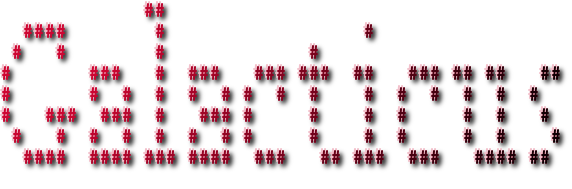
\includegraphics[width=125mm]{GalacticusLogo.png}\\

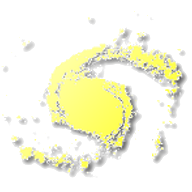
\includegraphics{New_Logo_Galaxy_192_Transparent.png}\\
A semi-analytic galaxy formation code.\\
Analyzing Galacticus Outputs Using Perl.\\

\copyright\ 2009, 2010 2011, 2012, 2013, 2014, 2015, 2016, 2017, 2018, 2019 Andrew Benson
\end{center}

\tableofcontents

\mainmatter
\pagestyle{headings}

\chapter{About Galacticus}

\glc\ is a semi-analytic model of galaxy formation. This document describes a collection of modules implemented in Perl designed for interacting with and analyzing the output of \glc\ models.

\subsection{License}

Copyright 2009, 2010, 2011, 2012, 2013, 2014, 2015, 2016, 2017, 2018, Andrew Benson \href{mailto:abenson@carnegiescience.edu}{\normalfont \ttfamily <abenson@carnegiescience.edu>}\\

\glc\ is free software: you can redistribute it and/or modify
it under the terms of the GNU General Public License as published by
the Free Software Foundation, either version 3 of the License, or
(at your option) any later version.

\glc\ is distributed in the hope that it will be useful,
but WITHOUT ANY WARRANTY; without even the implied warranty of
MERCHANTABILITY or FITNESS FOR A PARTICULAR PURPOSE.  See the
GNU General Public License for more details.

You should have received a copy of the GNU General Public License
along with \glc.  If not, see \href{http://www.gnu.org/licenses/}{\normalfont \ttfamily <http://www.gnu.org/licenses/>}.


\chapter{Extracting and Analyzing Results}

\glc\ stores its output in an \href{http://www.hdfgroup.org/HDF5/}{HDF5} file. The contents of this file can be viewed and manipulated using a variety of ways including:
\begin{description}
 \item[\href{http://www.hdfgroup.org/hdf-java-html/hdfview/}{{\normalfont \scshape HDFView}}] This is a graphical viewer for exploring the contents of HDF5 files;
 \item[\href{http://www.hdfgroup.org/products/hdf5_tools/index.html\#h5dist}{HDF5 Command Line Tools}] A set of tools which can be used to extract data from HDF5 files (\href{http://www.hdfgroup.org/HDF5/doc/RM/Tools.html#Tools-Dump}{{\normalfont \ttfamily h5dump}} and \href{http://www.hdfgroup.org/HDF5/doc/RM/Tools.html#Tools-Ls}{{\normalfont \ttfamily h5ls}} are particularly useful);
 \item[\href{http://www.hdfgroup.org/HDF5/doc/RM/RM_H5Front.html\#F90andCPPlus}{C++ and Fortran 90 APIs}] Allow access to and manipulation of data in HDF5 files;
 \item[\href{http://code.google.com/p/h5py/}{{\normalfont \scshape h5py}}] A Python interface to HDF5 files.
\end{description}

In the remainder of this section the structure of \glc\ HDF5 files is described and a general-purpose Perl module which we use to extract data in a convenient manner is outlined.

\section{General Structure of Output File}

Figure~\ref{fig:glcOutputFileStructure} shows the structure of a typical \glc\ output file. The various groups and subgroups are described below.

\begin{figure}
\begin{center}
\begin{verbatim}
outputFile.hdf5
 |
 +-> UUID                                     Attribute {1}
 |
 +-> Build                                    Group
 |    |
 |    +-> FGSL_library_version                Attribute {1}
 |    +-> FoX_library_version                 Attribute {1}
 |    +-> GSL_library_version                 Attribute {1}
 |    +-> HDF5_library_version                Attribute {1}
 |    +-> make_CCOMPILER                      Attribute {1}
 |    +-> make_CCOMPILER_VERSION              Attribute {1}
 |    +-> make_CFLAGS                         Attribute {1}
 |    +-> make_CPPCOMPILER                    Attribute {1}
 |    +-> make_CPPCOMPILER_VERSION            Attribute {1}
 |    +-> make_CPPFLAGS                       Attribute {1}
 |    +-> make_FCCOMPILER                     Attribute {1}
 |    +-> make_FCCOMPILER_VERSION             Attribute {1}
 |    +-> make_FCFLAGS                        Attribute {1}
 |    +-> make_FCFLAGS_NOOPT                  Attribute {1}
 |    +-> make_MODULETYPE                     Attribute {1}
 |    +-> make_PREPROCESSOR                   Attribute {1}
 |    +-> sourceChangeSetDiff                 Dataset   {1}
 |    +-> sourceChangeSetMerge                Dataset   {1}
 |
 +-> Outputs                                  Group
 |    |
 |    +-> Output1                             Group
 |    |    |
 |    |    +-> nodeData                       Group
 |    |    |     |
 |    |    |     +-> nodeProperty1            Dataset {<nodeCount>}
 |    |    |     +-> ...                      Dataset {<nodeCount>}
 |    |    |     +-> ...                      Dataset {<nodeCount>}
 |    |    |     +-> ...                      Dataset {<nodeCount>}
 |    |    |     +-> nodePropertyN            Dataset {<nodeCount>}
 |    |    |
 |    |    +-> mergerTreeCount                Dataset {<treeCount>}
 |    |    |
 |    |    +-> mergerTreeIndex                Dataset {<treeCount>}
 |    |    |
 |    |    +-> mergerTreeStartIndex           Dataset {<treeCount>}
 |    |    |
 |    |    +-> mergerTreeWeight               Dataset {<treeCount>}
 |    |    |
 |    |    +-> mergerTree1                    Group              [optional]
 |    |    |     |
 |    |    |     +-> nodeProperty1            Reference
 |    |    |     +-> ...                      Reference
 |    |    |     +-> ...                      Reference
 |    |    |     +-> ...                      Reference
 |    |    |     +-> nodePropertyN            Reference
 |    |    |
 |    |    x-> ...                            Group              [optional]
 |    |    x-> ...                            Group              [optional]
 |    |    x-> ...                            Group              [optional]
 |    |    x-> mergerTree<treeCount>          Group              [optional]
 |    |    |
 |    |    +-> outputExpansionFactor          Attribute {1}
 |    |    +-> outputTime                     Attribute {1}
 |    |
 |    x-> Output2                             Group
 |
 +-> Filters                                  Group
 |    |
 |    +-> name                                Dataset   {<filterCount>}
 |    +-> wavelengthEffective                 Dataset   {<filterCount>}
 |
 +-> Parameters                               Group
 |    |
 |    +-> inputParameter1                     Attribute {}
 |    +-> ...                                 Attribute {}
 |    +-> ...                                 Attribute {}
 |    +-> ...                                 Attribute {}
 |    +-> inputParameterN                     Attribute {}
 |    +-> inputParameter1                     Group
 |         |
 |         +-> subInputParameter1             Attribute {}
 |         +-> ...                            Attribute {}
 |         +-> subInputParameterN             Attribute {}
 |    x-> ...                                 Attribute {}
 |    x-> ...                                 Attribute {}
 |    x-> ...                                 Attribute {}
 |    x-> inputParameterN                     Group
 |
 +-> Version                                  Group
 |    |
 |    +-> runTime                             Attribute {1}
 |    +-> versionMajor                        Attribute {1}
 |    +-> versionMinor                        Attribute {1}
 |    +-> versionRevision                     Attribute {1}
 |    +-> hgRevision                          Attribute {1}
 |    +-> hgHash                              Attribute {1}
 |    +-> runByName                           Attribute {1}
 |    +-> runByEmail                          Attribute {1}
 |
 +-> globalHistory                            Group
      |
      +-> historyExpansion                    Dataset {<historyCount>}
      +-> historyStarFormationRate            Dataset {<historyCount>}
      +-> historyTime                         Dataset {<historyCount>}
\end{verbatim}
\end{center}
\caption{Structure of a \glc\ HDF5 output file. {\normalfont \ttfamily <treeCount>} is the total number of merger trees present in a given output, and {\normalfont \ttfamily <nodeCount} is the total number of nodes (in all trees) present in an output.}
\label{fig:glcOutputFileStructure}
\end{figure}

\subsection{UUID}\label{sec:UUID}

The UUID (\href{https://secure.wikimedia.org/wikipedia/en/wiki/Universally_unique_identifier}{Universally Unique Identifier}) is a unique identifier assigned to each \glc\ model that is run. It allows identification of a given model and can be referenced from, for example, an external database. Using the {\normalfont \ttfamily Galacticus::HDF5} Perl module (see \S\ref{sec:perlModuleDataExtraction}), the UUID can be loaded into the data structure using:
\begin{verbatim}
&HDF5::Get_UUID($model);
\end{verbatim}
The UUID is then available as {\normalfont \ttfamily \$model-\textgreater\{'uuid'\}}.

\subsection{Build Information}\label{sec:BuildInformation}

\glc\ automatically stores various information about how it was built in the {\normalfont \ttfamily Build} group attributes. Currently, included attributes consist of:
\begin{description}
\item[{\normalfont \ttfamily FGSL\_library\_version}] The version number of the FGSL library;
\item[{\normalfont \ttfamily FoX\_library\_version}] The version number of the FoX library;
\item[{\normalfont \ttfamily GSL\_library\_version}] The version number of the GSL library;
\item[{\normalfont \ttfamily HDF5\_library\_version}] The version number of the HDF5 library;
\item[{\normalfont \ttfamily make\_CCOMPILER}] The C compiler command used;
\item[{\normalfont \ttfamily make\_CCOMPILER\_VERSION}] The C compiler version information;
\item[{\normalfont \ttfamily make\_CFLAGS}] The flags passed to the C compiler;
\item[{\normalfont \ttfamily make\_CPPCOMPILER}] The C++ compiler command used;
\item[{\normalfont \ttfamily make\_CPPCOMPILER\_VERSION}] The C++ compiler version information;
\item[{\normalfont \ttfamily make\_CPPFLAGS}] The flags passed to the C++ compiler;
\item[{\normalfont \ttfamily make\_FCCOMPILER}] The Fortran compiler command used;
\item[{\normalfont \ttfamily make\_FCCOMPILER\_VERSION}] The Fortran compiler version information;
\item[{\normalfont \ttfamily make\_FCFLAGS}] The flags passed to the Fortran compiler;
\item[{\normalfont \ttfamily make\_FCFLAGS\_NOOPT}] The flags passed to the Fortran compiler for unoptimized compiles;
\item[{\normalfont \ttfamily make\_MODULETYPE}] The Fortran module type identifier string;
\item[{\normalfont \ttfamily make\_PREPROCESSOR}] The preprocessor command used.
\end{description}

Additionally, two datasets are included which store details of the \glc\ source changeset. {\normalfont \ttfamily sourceChangeSetMerge} contains the output of ``{\normalfont \ttfamily hg bundle -t none}'', that is, it contains a Mercurial changegroup that incorporates any changes made to the current branch relative to the main \glc\ branch. {\normalfont \ttfamily sourceChangeSetDiff} contains the output of ``{\normalfont \ttfamily hg diff}'', that is, all differences between the source code in the working directory and that which has been committed to Mercurial. Used together, these two datasets allow the precise source code used to run the model to be recovered from the main branch \glc\ source.

\subsection{Filters}

For each broadband filter used in the \glc\ model run an entry is added to the datasets in this group. Currently, two datasets are generated:
\begin{description}
\item[{\normalfont \ttfamily name}] The name of each filter used.
\item[{\normalfont \ttfamily wavelengthEffective}] The effective wavelength, $\lambda_\mathrm{eff}$ (defined as $\lambda_\mathrm{eff}=\left. \int_0^\infty \lambda R(\lambda) \mathrm{d}\lambda \right/ \int_0^\infty R(\lambda) \mathrm{d}\lambda$, where $R(\lambda)$ is the filter response) of the filter in \AA.
\end{description}

\subsection{Parameters}

The {\normalfont \ttfamily Parameters} group contains a record of all parameter values (either input or default) that were used for this \glc\ run. The group contains a long list of attributes, each attribute named for the corresponding parameter and with a single entry giving the value of that parameter. If a parameter has subparameters, a group is created having the same name as the parameter, which will contain attributes corresponding to each subparameter. The {\normalfont \ttfamily scripts/aux/Extract\_Parameter\_File.pl} script can be used to extract these parameter values to an XML file suitable for re-input into \glc.

\subsection{Version}

The {\normalfont \ttfamily Version} group contains a record of the \glc\ version used for this model, storing the major and minor version numbers, the revision number and the {\normalfont \scshape Mercurial} revision and hash (if the code is being maintained using {\normalfont \scshape Mercurial}, otherwise a value of $-1$ is entered or the revision and the hash attribute is empty). Additionally, the time at which the model was run is stored and, if the {\normalfont \ttfamily galacticusConfig.xml} file (see \S\ref{sec:ConfigFile}) is present and contains contact details, the name and e-mail address of the person who ran the model.

\subsection{globalHistory}\label{sec:globalHistory}\index{history!global}\index{outputs!global history}

The {\normalfont \ttfamily globalHistory} group stores volume averaged properties of the model universe as a function of time. Currently, the properties stored are:
\begin{description}
 \item[{\normalfont \ttfamily historyTime}] Cosmic time (in Gyr);
 \item[{\normalfont \ttfamily historyExpansion}] Expansion factor;
 \item[{\normalfont \ttfamily historyStarFormationRate}] Volume averaged star formation rate (in $M_\odot/$Gyr/Mpc$^3$).
 \item[{\normalfont \ttfamily historyDiskStarFormationRate}] Volume averaged star formation rate in disks (in $M_\odot/$Gyr/Mpc$^3$).
 \item[{\normalfont \ttfamily historySpheroidStarFormationRate}] Volume averaged star formation rate in spheroids (in $M_\odot/$Gyr/Mpc$^3$).
 \item[{\normalfont \ttfamily historyStellarDensity}] Volume averaged stellar mass density (in $M_\odot/$Mpc$^3$).
 \item[{\normalfont \ttfamily historyDiskStellarDensity}] Volume averaged stellar mass density in disks (in $M_\odot/$Mpc$^3$).
 \item[{\normalfont \ttfamily historySpheroidStellarDensity}] Volume averaged stellar mass density in spheroids (in $M_\odot/$Mpc$^3$).
 \item[{\normalfont \ttfamily historyGasDensity}] Volume averaged cooled gas density (in $M_\odot/$Mpc$^3$).
 \item[{\normalfont \ttfamily historyNodeDensity}] Volume averaged resolved node density (in $M_\odot/$Mpc$^3$).
\end{description}
Dimensionful datasets have a {\normalfont \ttfamily unitsInSI} attribute which gives their units\index{units} in the SI system.

\subsection{Outputs}

The {\normalfont \ttfamily Outputs} group contains one or more sub-groups corresponding to the output times requested from \glc. Each sub-group contains the following information:
\begin{description}
 \item[{\normalfont \ttfamily outputTime} \emph{(attribute)}] The cosmic time (in Gyr) at this output;
 \item[{\normalfont \ttfamily outputExpansionFactor} \emph{(attribute)}] The expansion factor at this output;
 \item[{\normalfont \ttfamily nodeData}] A group of node properties as described below.
 \item[{\normalfont \ttfamily mergerTree} subgroups \emph{(optional)}] A set of {\normalfont \ttfamily mergerTree} groups as described below.
\end{description}

Output is controlled by parameters given within the {\normalfont \ttfamily mergerTreeOutput} section of the parameter file. Current options are:
\begin{description}
\item[{\normalfont \ttfamily outputMergerTrees}] If {\normalfont \ttfamily true} then each merger tree is output to the relevant sub-group at each output time (see \S\ref{sec:nodeDataGroup}). Otherwise merger trees are not output. [Default: {\normalfont \ttfamily true}.]
\item[{\normalfont \ttfamily outputReferences}] If {\normalfont \ttfamily true} then an HDF5 reference dataset is written for each merger tree subgroup (see \S\ref{sec:mergerTreeSubgroups}). [Default: {\normalfont \ttfamily false}.]
\item[{\normalfont \ttfamily galacticFilterMethod}] A ``galactic filter'' (see \S\ref{sec:methodsGalacticFilter}) which is applied to each node in the tree to determine whether or not it should be output. By combinding multiple filters it is possible to construct arbitrarily complex criteria for output. [Default: {\normalfont \ttfamily always}.]
\end{description}

\subsubsection{nodeData group}\label{sec:nodeDataGroup}

The {\normalfont \ttfamily nodeData} group contains all data from nodes in all merger trees. The group consists of a collection of datasets each of which lists a property of all nodes in the trees which exist at the output time. Where relevant, each dataset contains an attribute, {\normalfont \ttfamily unitsInSI}, which gives the units\index{units} of the dataset in the SI system.

\subsubsection{mergerTree datasets}\label{sec:mergerTreeDatasets}

To allow locating of nodes belonging to a given merger tree in the datasets in the {\normalfont \ttfamily nodeData} group, the {\normalfont \ttfamily mergerTreeStartIndex} and {\normalfont \ttfamily mergerTreeCount} datasets list the starting index of each tree's nodes in the {\normalfont \ttfamily nodeData} datasets, and the number of nodes belonging to each tree respectively. Additionally, the {\normalfont \ttfamily mergerTreeWeight} dataset lists the {\normalfont \ttfamily volumeWeight} property for each tree (see \S\ref{sec:mergerTreeSubgroups}) which gives the weight (in Mpc$^{-3}$) which should be assigned to this tree (and all nodes in it) to create a volume-averaged sample (see \S\ref{sec:volumeLimitedSamples}). Finally, the {\normalfont \ttfamily mergerTreeIndex} dataset gives the index of each tree stored in the {\normalfont \ttfamily nodeData} datasets.

\subsubsection{mergerTree subgroups}\label{sec:mergerTreeSubgroups}

These subgroups will be present if the {\normalfont \ttfamily [mergerTreeOutputReferences]} parameter is set to true. Each {\normalfont \ttfamily mergerTree} subgroup contains HDF5 references to all data on a single merger tree. The group consists of a collection of scalar references each of which points to the appropriate region of the corresponding dataset in the {\normalfont \ttfamily nodeData} group. Additionally, the {\normalfont \ttfamily volumeWeight} attribute of this group gives the weight (in Mpc$^{-3}$) which should be assigned to this tree (and all nodes in it) to create a volume-averaged sample. (A second attribute, {\normalfont \ttfamily volumeWeightUnitsInSI}, gives the units of {\normalfont \ttfamily volumeWeight} in the SI system.)

\subsection{Optional Outputs}

Numerous other quantities can be optionally output. These are documented below:

\subsubsection{Redshifts}\index{redshift!output}\index{output!redshift}

The redshift corresponding to the time at which a node was last isolated can be output by setting {\normalfont \ttfamily [outputNodeRedshifts]} to {\normalfont \ttfamily true}. This quantity will be output as {\normalfont \ttfamily basicRedshiftLastIsolated}.

\subsubsection{Mass Accretion Histories}

A mass accretion history (i.e. mass as a function of time) for the main branch in each merger tree can be output by setting {\normalfont \ttfamily massAccretionHistoryOutput}$=${\normalfont \ttfamily true}. If requested, a new group {\normalfont \ttfamily massAccretionHistories} will be made in the \glc\ output file. It will contain groups called {\normalfont \ttfamily mergerTreeN} where {\normalfont \ttfamily N} is the merger tree index. Each such group will contain the following three datasets, defined for the main branch of the tree\footnote{``Main branch'' is defined by starting from the root node of a tree and repeatedly stepping back to the most massive progenitor of the branch. This does not necessarily pick out the most massive progenitor at a given time.}:
\begin{description}
 \item [{\normalfont \ttfamily nodeIndex}] The index of the node in the tree;
 \item [{\normalfont \ttfamily nodeTime}] The time at this point in the tree (in Gyr);
 \item [{\normalfont \ttfamily nodeMass}] The mass of the node at this point in the tree (in $M_\odot$). The {\normalfont \ttfamily nodeMass} property is defined to be the total mass of each node in a merger tree. Therefore, it includes both dark and baryonic mass. Additionally, the mass of a node includes the mass of any satellite nodes that it may contain. The mean density of the node depends on the method selected by the {\normalfont \ttfamily virialDensityContrastMethod} parameter.
\end{description}

\subsubsection{Merger Tree Dump}

A full dump of merger tree structure by setting {\normalfont \ttfamily mergerTreeStructureDump}$=${\normalfont \ttfamily true}. In this case, files will be dumped to the directory specified by {\normalfont \ttfamily [mergerTreeStructureDumpDirectory]} for each merger tree with final mass between {\normalfont \ttfamily [mergerTreeStructureDumpMassMinimum]} and {\normalfont \ttfamily [mergerTreeStructureDumpMassMaximum]}. Each tree is dumped to a file named ``{\normalfont \ttfamily mergerTreeDump:\textless treeIndex\textgreater:1.gv}'' in the specified directory in {\normalfont \scshape GraphViz} format.

\subsubsection{Conditional Mass Functions}

Setting {\normalfont \ttfamily [mergerTreeComputeConditionalMassFunction]}$=${\normalfont \ttfamily true} will cause conditional mass functions to be computed and output to the \glc\ output file in a group named ``{\normalfont \ttfamily conditionalMassFunction}''. The mass functions are binned in parent halo mass, and the mass ratio of the progenitor to parent halo. Bins are logarithmically spaced in mass (and mass ratio), with the range and number of bins controlled by the parameters:
\begin{itemize}
\item {\normalfont \ttfamily [mergerTreeComputeConditionalMassFunctionParentMassCount]};
\item {\normalfont \ttfamily [mergerTreeComputeConditionalMassFunctionParentMassMinimum]};
\item {\normalfont \ttfamily [mergerTreeComputeConditionalMassFunctionParentMassMaximum]};
\item {\normalfont \ttfamily [mergerTreeComputeConditionalMassFunctionMassRatioCount]};
\item {\normalfont \ttfamily [mergerTreeComputeConditionalMassFunctionMassRatioMinimum]};
\item {\normalfont \ttfamily [mergerTreeComputeConditionalMassFunctionMassRatioMaximum]}.
\end{itemize}
The resulting parent masses and mass ratios are written to datasets {\normalfont \ttfamily massParent} and {\normalfont \ttfamily massRatio} respectively. Parent and progenitor halos are defined at a set of redshifts defined by the arrays {\normalfont \ttfamily [mergerTreeComputeConditionalMassFunctionParentRedshifts]}, and {\normalfont \ttfamily [mergerTreeComputeConditionalMassFunctionProgenitorRedshifts]}, which are written to datasets {\normalfont \ttfamily redshiftParent} and {\normalfont \ttfamily redshiftProgenitor}. The resulting conditional masses functions are written to datasets {\normalfont \ttfamily conditionalMassFunction} and {\normalfont \ttfamily conditionalMassFunctionError}.

In addition to standard progenitor mass functions, the progenitor mass function conditioned on progenitor rank (i.e. 1$^\mathrm{st}$ most massive, 2$^\mathrm{nd}$, \ldots, $n^\mathrm{th}$ most massive progenitor) is computed and output to the datasets {\normalfont \ttfamily primaryProgenitorMassFunction} and {\normalfont \ttfamily primaryProgenitorMassFunctionError}. The depth (i.e. $n$) is specifed by {\normalfont \ttfamily [mergerTreeComputeConditionalMassFunctionPrimaryProgenitorDepth]}.

Finally, the progenitor mass functoin conditioned on recent formation is computed and output to the datasets {\normalfont \ttfamily formationRateFunction} and {\normalfont \ttfamily formationRateFunctionError}. To be considered ``recently formed'' a progenitor must have formed between $t$ and $t(1-\Delta)$ where $t$ is the progenitor time and $\Delta=${\normalfont \ttfamily [mergerTreeConditionalMassFunctionFormationRateTimeFraction]}.

\subsubsection{Pre-Evolution Merger Trees}

\glc\ can output the full structure of merger trees prior to any evolution. Merger tree structure can be requested by setting {\normalfont \ttfamily mergerTreeStructureOutput}$=${\normalfont \ttfamily true}. Structures are written to a new group, {\normalfont \ttfamily mergerTreeStructures}, in the \glc\ output file. This group will contain groups called {\normalfont \ttfamily mergerTreeN} where {\normalfont \ttfamily N} is the merger tree index. Each such group will contain the following datasets:
\begin{description}
 \item [{\normalfont \ttfamily nodeIndex}] The index of the node in the tree;
 \item [{\normalfont \ttfamily childIndex}] The index of this node's first child node;
 \item [{\normalfont \ttfamily parentIndex}] The index of this node's parent node;
 \item [{\normalfont \ttfamily siblingIndex}] The index of this node's sibling node;
 \item [{\normalfont \ttfamily nodeTime}] The time at this point in the tree (in Gyr);
 \item [{\normalfont \ttfamily nodeMass}] The mass of the node at this point in the tree (in $M_\odot$). The {\normalfont \ttfamily nodeMass} property is defined to be the total mass of each node in a merger tree. Therefore, it includes both dark and baryonic mass. Additionally, the mass of a node includes the mass of any satellite nodes that it may contain. The mean density of the node depends on the method selected by the {\normalfont \ttfamily virialDensityContrastMethod} parameter.
\end{description}
Additional, optional, datasets can be added by setting appropriate input parameters. Currently these include:
\begin{itemize}
 \item [Virial quantities] If {\normalfont \ttfamily mergerTreeStructureOutputVirialQuantities}$=${\normalfont \ttfamily true} then two additional datasets are included:
 \begin{description}
  \item [{\normalfont \ttfamily nodeVirialRadius}] The virial radius of the node (in Mpc);
  \item [{\normalfont \ttfamily nodeVirialVelocity}] The virial velocity of the node (in km/s);
 \end{description}
 \item [Dark matter scale radii] If {\normalfont \ttfamily mergerTreeStructureOutputDarkMatterScaleRadius}$=${\normalfont \ttfamily true} then an additional dataset is included:
 \begin{description}
  \item [{\normalfont \ttfamily darkMatterScaleRadius}] The scale radius of this node's dark matter halo profile (in Mpc);
 \end{description}
 \item [Merger tree final descendent] If {\normalfont \ttfamily outputFinalDescendentIndices}$=${\normalfont \ttfamily true} then an additional dataset is included:
 \begin{description}
  \item [{\normalfont \ttfamily finalDescendentIndex}] The index of the final descendent that this node will reach in its merger trees;
 \end{description}
\end{itemize}

\section{Perl Module for Data Extraction}\label{sec:perlModuleDataExtraction}

A Perl module is provided that allows for easy extraction of datasets from the \glc\ output file together with a straightforward way to implement derived properties. To use this Perl module, add
\begin{verbatim}
 use lib "./perl";
 use PDL;
 use Galacticus::HDF5;
\end{verbatim}
at the start of your Perl script. The {\normalfont \ttfamily Galacticus::HDF5} module will import data from a \glc\ HDF5 file into PDL variables. All data are stored in a single structure, which also specifies the file, output and range of trees to read. An example of reading a dataset from a file is:
\begin{verbatim}
 my $model;
 $model->{'file'     } = "galacticus.hdf5";
 $model->{'output'   } = 1;
 $model->{'tree'     } = "all";
 $model->{'dataRange'} = [1,2];
 $model->{'store'    } = 0;
 &HDF5::Get_Dataset($model,['nodeMass']);
 $dataSets = $model->{'dataSets'};
 print $dataSets->{'nodeMass'}."\n";
\end{verbatim}
The {\normalfont \ttfamily \$model} object is initialized with information to specify which file, output and trees should be used. Its settable components are:
\begin{description}
 \item [{\normalfont \ttfamily file}] The name of the \glc\ output file to be read.
 \item [{\normalfont \ttfamily output}] Specify the output number in the file which should be read.
 \item [{\normalfont \ttfamily tree}] Specify the tree which should be read, or use ``all'' to specify that all trees be read.
 \item [{\normalfont \ttfamily dataRange}] Gives the first and last entry in the dataset to read---this facilitates reading of partial datasets (and therefore reading datasets in a piecemeal fashion). If this component is missing, the entire dataset is read.
 \item[{\normalfont \ttfamily store}] If set to 1, any derived properties will be stored back in the \glc\ output file for later retrieval. If set to 0 (or if this option is not present), derived properties will not be stored. Currently, storing of derived properties in the \glc\ file is only possible if the {\normalfont \ttfamily tree} option is set to ``all'' and no {\normalfont \ttfamily dataRange} is specified.
\end{description}
The {\normalfont \ttfamily \&HDF5::Get\_Dataset(\$model,['nodeMass']);} call requests that the {\normalfont \ttfamily nodeMass} dataset be read. It is return as a PDL variable in the {\normalfont \ttfamily nodeMass} element of the {\normalfont \ttfamily dataSets} element which is itself a member of {\normalfont \ttfamily \$model}. The final lines in the example simply write out the resulting array of {\normalfont \ttfamily nodeMass} values.

\subsection{Derived Properties}

Derived properties can be created by giving defining functions along with a regular expression string that allows them to be matched. For example, the {\normalfont \ttfamily Galacticus::Baryons} module implements a hot gas fraction property called {\normalfont \ttfamily hotHaloFraction} or {\normalfont \ttfamily hotHaloFrac}. It has the following form:
\begin{verbatim}
package Baryons;
use PDL;
use Galacticus::HDF5;
use Data::Dumper;

%HDF5::galacticusFunctions = ( %HDF5::galacticusFunctions,
    "hotHalo(Fraction|Frac)" => \&Baryons::Get_hotHaloFraction
    );

my $status = 1;
$status;

sub Get_hotHaloFraction {
    $model = shift;
    $dataSetName = $_[0];
    &HDF5::Get_Dataset($model,['hotHaloMass','nodeMass']);
    $dataSets = $model->{'dataSets'};
    $dataSets->{$dataSetName} = $dataSets->{'hotHaloMass'}/$dataSets->{'nodeMass'};
}

\end{verbatim}
The module begins by adding an entry to the {\normalfont \ttfamily \%HDF5::galacticusFunctions} hash. The key gives a regular expression which matches to the name of the property to be defined. The value of the key gives a reference to a subroutine to be called to evaluate this expression. The subroutine is defined below. When called, it receives the {\normalfont \ttfamily \$model} structure along with the name of the requested property. The subroutine should then simply evaluate the requested property and store it in the appropriate location within {\normalfont \ttfamily \$model}. Note that the subroutine can request additional datasets be loaded (as happens above where {\normalfont \ttfamily hotHaloMass} and {\normalfont \ttfamily nodeMass} are requested) if they are needed for its calculations.

\subsubsection{Available Derived Properties}\label{sec:DerivedProperties}

\begin{description}
 \item[{\normalfont \ttfamily mergerTreeIndex}] The index of the merger tree in which the galaxy is found. Provided by: {\normalfont \ttfamily Galacticus::HDF5}.
 \item[{\normalfont \ttfamily redshift}] The redshift at which the galaxy exists. Provided by: {\normalfont \ttfamily Galacticus::Time}.
 \item[{\normalfont \ttfamily time}] The cosmic time (in Gyr) at which the galaxy exists. Provided by: {\normalfont \ttfamily Galacticus::Time}.
 \item[{\normalfont \ttfamily expansionFactor}] The expansion factor at which the galaxy exists. Provided by: {\normalfont \ttfamily Galacticus::Time}.
 \item[{\normalfont \ttfamily stellarMass}] The sum of disk and spheroid stellar masses. Provided by: {\normalfont \ttfamily Galacticus::StellarMass}.
 \item[{\normalfont \ttfamily massColdGas}] The sum of disk and spheroid cold gas masses. Provided by: {\normalfont \ttfamily Galacticus::GasMass}.
 \item[{\normalfont \ttfamily starFormationRate}] The sum of disk and spheroid star formation rates. Provided by: {\normalfont \ttfamily Galacticus::StellarMass}.
 \item[{\normalfont \ttfamily hostNodeMass}] For isolated nodes, the node mass. For non-isolated nodes, the mass of the isolated node in which the node resides. Provided by: {\normalfont \ttfamily Galacticus::HostNode}.\index{nodes!host mass}\index{halos!host mass}\index{satellites!host mass}
 \item[{\normalfont \ttfamily stellarMass}] The sum of disk and speheroid stellar masses (or, whichever of these exist in the model). Provided by: {\normalfont \ttfamily Galacticus::StellarMass}.
 \item[{\normalfont \ttfamily hotHalo(Fraction\textbar Frac)}] The fraction the node's mass in the hot gas halo. Provided by: {\normalfont \ttfamily Galacticus::Baryons}.
 \item[{\normalfont \ttfamily inclination}] A randomly selected inclination for the disk (in degrees). Provided by: {\normalfont \ttfamily Galacticus::Inclination}.
 \item[{\normalfont \ttfamily \textasciicircum(disk\textbar bulge)StellarLuminosity:.*:dustAtlas($\backslash$[faceOn$\backslash$])\$}] Dust-extingiushed\index{dust!extinction} luminosities for disk and bulge found by interpolating in the dust tables of \cite{ferrara_atlas_1999}. If the {\normalfont \ttfamily [faceOn]} qualifier is present, extinctions are computed assuming that the disk is observed face-on, otherwise a random inclination is used. Optionally, the dust atlas file to used can be specified via {\normalfont \ttfamily \$dataSet-\textgreater\{'dustAtlasFile'\}}. The available dust atlases span a limited range of spheroid sizes and central optical depths in their tabulations. Standard behavior is to extrapolate beyond the ends of these ranges. This can be controlled via {\normalfont \ttfamily \$dataSet-\textgreater\{'dustAtlasExtrapolateInSize'\}} and {\normalfont \ttfamily \$dataSet-\textgreater\{'dustAtlasExtrapolateInTau'\}} respectively, which can be set to {\normalfont \ttfamily yes}/{\normalfont \ttfamily no} (or, equivalently, 1/0). \emph{Note:} Dust attenuated luminosities for all galaxies, all filters, and all output redshifts can be computed and stored back to the \gls{hdf5} file using a simple script as described in \S\ref{sec:TutorialDustAttenuation}. Provided by: {\normalfont \ttfamily Galacticus::DustAttenuation}.
 \item[{\normalfont \ttfamily \textasciicircum(disk\textbar bulge)LuminositiesStellar:.*:dustCharlotFall2000\$}] Dust-extingiushed\index{dust!extinction} luminosities for disk and bulge found using the model of \cite{charlot_simple_2000}. Provided by: {\normalfont \ttfamily Galacticus::DustCharlotFall2000}.
 \item[{\normalfont \ttfamily \textasciicircum totalStellarLuminosity:.*:dustAtlas($\backslash$[faceOn$\backslash$])\$}] (Optionally dust-extingiushed) luminosities for disk plus bulge found by adding together the corresponding disk and bulge luminosities. Provided by: {\normalfont \ttfamily Galacticus::Luminosities}.
 \item[{\normalfont \ttfamily \textasciicircum bulgeToTotalLuminosity:.*:dustAtlas($\backslash$[faceOn$\backslash$])\$}] Ratio of bulge to total (optionally dust-extingiushed) luminosities. Provided by: {\normalfont \ttfamily Galacticus::Luminosities}.
 \item[{\normalfont \ttfamily \textasciicircum magnitude([\textasciicircum :]+):([\textasciicircum :]+):([\textasciicircum :]+):z([$\backslash$d$\backslash$.]+)(:dust[\textasciicircum :]+)?(:vega\textbar :AB)?}] Absolute magnitude corresponding to a stellar luminosity, in either Vega or AB systems. Provided by: {\normalfont \ttfamily Galacticus::Magnitudes}.
 \item[{\normalfont \ttfamily \textasciicircum magnitude:(.*)(:vega\textbar :AB)?}] Absolute magnitude corresponding to the generic luminosity property {\normalfont \ttfamily \textasciicircum luminosity:\$1}, in either Vega or AB systems. Provided by: {\normalfont \ttfamily Galacticus::Magnitudes}.
 \item[{\normalfont \ttfamily \textasciicircum apparentMagnitude:(.*)}] Apparent magnitude corresponding to the absolute magnitude {\normalfont \ttfamily \textasciicircum magnitude:\$1}. Provided by: {\normalfont \ttfamily Galacticus::Magnitudes}.
 \item[{\normalfont \ttfamily comovingDistance}] The comoving distance (in Mpc) to the galaxy---provided by {\normalfont \ttfamily Galacticus::Survey} (see \S\ref{sec:Galacticus::Survey} for a full description).
 \item[{\normalfont \ttfamily luminosityDistance}] The luminosity distance (in Mpc) to the galaxy---provided by {\normalfont \ttfamily Galacticus::Survey} (see \S\ref{sec:Galacticus::Survey} for a full description).
 \item[{\normalfont \ttfamily distanceModulus}] The distance modulus (including the $+2.5\log_{10}(1+z)$ term to account for squeezing of photon frequencies) to the galaxy---provided by {\normalfont \ttfamily Galacticus::Survey} (see \S\ref{sec:Galacticus::Survey} for a full description).
 \item[{\normalfont \ttfamily redshift}] The redshift at which the galaxy is observed---provided by {\normalfont \ttfamily Galacticus::Survey} (see \S\ref{sec:Galacticus::Survey} for a full description).
 \item[{\normalfont \ttfamily angularWeight}] The weight (in units of ) which should be assigned to this galaxy in order to build a redshift survey---provided by {\normalfont \ttfamily Galacticus::Survey} (see \S\ref{sec:Galacticus::Survey} for a full description).
 \item[{\normalfont \ttfamily angularDiameterDistance}] The angular diameterer distance (in Mpc) to the galaxy---provided by {\normalfont \ttfamily Galacticus::Survey} (see \S\ref{sec:Galacticus::Survey} for a full description).
 \item[{\normalfont \ttfamily \textasciicircum angularPosition[12]}] The angular position (in radians measured along two orthogonal axes from the center of the field) of the galaxy---provided by {\normalfont \ttfamily Galacticus::Survey} (see \S\ref{sec:Galacticus::Survey} for a full description).
 \item[{\normalfont \ttfamily \textasciicircum grasilFlux[$\backslash$d$\backslash$.]+microns}] The flux at the given wavelength (specific in microns) of the galaxy as computed by the {\normalfont \ttfamily Grasil} code (see \S\ref{sec:Grasil} for a full description).
 \item[{\normalfont \ttfamily \textasciicircum grasilInfraredLuminosity}] The total infrared (8--1000$\mu$m) luminosity of the galaxy as computed by the {\normalfont \ttfamily Grasil} code (see \S\ref{sec:Grasil} for a full description).
 \item[{\normalfont \ttfamily \textasciicircum grasilFlux:([\textasciicircum :]+)}] The flux (in Janskys) of the galaxy as computed by the {\normalfont \ttfamily Grasil} code integrated under the specified filter (see \S\ref{sec:Grasil} for a full description).
 \item[{\normalfont \ttfamily \textasciicircum luminosity:grasil:([\textasciicircum :]+):([\textasciicircum :]+)}] The luminosity (in units of the zero point of the AB magnitude system) of the galaxy as computed by the {\normalfont \ttfamily Grasil} code integrated under the specified filter and in the specified frame (see \S\ref{sec:Grasil} for a full description).
 \item[{\normalfont \ttfamily flux850micronHayward}] The flux of the galaxy at 850$\mu$m\index{flux!sub-mm} computed using the fitting formula of \cite{hayward_what_2010}, specifically:
\begin{equation}
 {S_{850\mu\mathrm{m}} \over \mathrm{Jy}} = A \left({\dot{M}_\star \over 100 M_\odot \hbox{Gyr}^{-1}}\right)^\alpha \left({R_\mathrm{dust} M_\mathrm{metals,gas} \over 10^8 M_\odot}\right)^\beta,
\end{equation}
where $R_\mathrm{dust}$ is the dust-to-metals ratio, $\dot{M}_\star$ is the total star formation rate in the galaxy and $M_\mathrm{metals,gas}$ is the total mass of metals in the gas phase of the galaxy. Note that the fit given by \cite{hayward_what_2010} was computed for galaxcy at $z\approx 2$. The parameters of the fit can be specified by setting elements of {\normalfont \ttfamily \$model-\textgreater\{'haywardSubMmFit'\}}: {\normalfont \ttfamily \{'dustToMetalsRatio'\}}$\equiv R_\mathrm{dust}$, {\normalfont \ttfamily \{'fitNormalization'\}}$\equiv A$, {\normalfont \ttfamily \{'starFormationRateExponent'\}}$\equiv \alpha$, and {\normalfont \ttfamily \{'dustMassExponent'\}}$\equiv \beta$. If these elements are not present the default values of $A=0.65\times 10^{-3}$, $R_\mathrm{dust}=0.61$, $\alpha=0.42$ and $\beta = 0.58$ \cite{hayward_what_2010} will be used instead. Provided by: {\normalfont \ttfamily Galacticus::SubMmFluxesHayward}.
 \item[{\normalfont \ttfamily \textasciicircum(disk|spheroid|total)LymanContinuumLuminosity:z[$\backslash$d$\backslash$.]+\$}] The luminosity (in units of $10^{50}$photons/s) of the \gls{LymanContinuum} radiation of the disk or spheroid component, or total of the two at the specified redshift. The rest-frame {\normalfont \ttfamily Lyc} filter must have been computed in \glc\ to allow this luminosity to be computed. If the {\normalfont \ttfamily Lyc} filter was computed with a non-default postprocessing chain then the name of the chain should be specified in {\normalfont \ttfamily \$dataBlock-\textgreater\{'lymanContinuum'\}-\textgreater\{'postProcessingChain'\}} Provided by: {\normalfont \ttfamily Galacticus::Lyc}.\index{continuum radiation!Lyman continuum}\index{Lyman continuum}
 \item[{\normalfont \ttfamily \textasciicircum agnLuminosity:[\textasciicircum:]+:[\textasciicircum:]+:z[$\backslash$d$\backslash$.]+(:alpha[0-9$\backslash$-$\backslash$+$\backslash$.]+)??\$}] The luminosity of the AGN in the specified filter, frame and redshift (specified as the first, second and third elements of the ``{\normalfont \ttfamily :}'' separated label) in units of the zero-point luminosity of the AB-magnitude system. (Note that, consistent with \glc's definitions for continuum luminosities, observed frame luminosities do not include the $1+z$ factor arising from the compression of photon frequencies due to redshifting. As such, when observed frame line luminosities are converted to observed fluxes an additional multiplicative factor of $1+z$ must be included.) The bolometric luminosity is computed from the black hole rest mass accretion rate and radiative efficiency. An SED for an AGN of this bolometric luminosity is then computed using the model of \cite{hopkins_observational_2007}. If the final {\normalfont \ttfamily alpha[0-9$\backslash$-$\backslash$+$\backslash$.]+} option is provided, then the luminosity computed will be a broad band luminosity (in units of Watts) converted from the photon count rate in the filter assuming a spectrum of the form $f_\nu \propto \nu^\alpha$, as is typically assumed in converting observed AGN X-ray count rates to luminosities. Provided by: {\normalfont \ttfamily Galacticus::AGNLuminosities}.\index{AGN}


 \item[{\normalfont \ttfamily \textasciicircum columnDensity(disk|Spheroid)??\$}] The column density of hydrogen (in units of cm$^{-2}$) along the line of sight to the center of the galaxy. If a component is specified the calculation is performed for that component, otherwise the sum of disk and spheroid column densities is computed. Provided by: {\normalfont \ttfamily Galacticus::ColumnDensity}. For the exponential disk, the column density is given by:
\begin{equation}
N_\mathrm{H} = {X_\mathrm{H} \over m_\mathrm{H}} {M_\mathrm{ISM} \over 4 \pi h r_\mathrm{d}^3} \int_0^\infty \exp(-r/r_\mathrm{d}) \mathrm{sech}^2(z/h r_\mathrm{d}) \mathrm{d} l,
\end{equation}
where $r_\mathrm{d}$ is the disk scale length, $h$ is the ratio of vertical scale height to radial scale length, $X_\mathrm{H}$ is the mass fraction in hydrogen, $m_\mathrm{H}$ is the mass of the hydrogen atom and $l$ is distance along the line of sight. Writing $z = r/\tan i$ for a disk at inclination $i$, and $l = \sqrt{r^2+z^2} = r\sqrt{1+1/\tan^2i}$ this becomes:
\begin{equation}
N_\mathrm{H} = {X_\mathrm{H} \over m_\mathrm{H}} {M_\mathrm{ISM} \over 4 \pi h r_\mathrm{d}^2} \sqrt{1+1/\tan^2i} \int_0^\infty \exp(-x) \mathrm{sech}^2(x/h \tan i) \mathrm{d} x.
\end{equation}
The integral can be evaluated to give:
\begin{equation}
N_\mathrm{H} = {X_\mathrm{H} \over m_\mathrm{H}} {M_\mathrm{ISM} \over 8 \pi h r_\mathrm{d}^2} \sqrt{1+1/\tan^2i} H \left\{ H \left[\psi\left(-{H\over4}\right) - \psi\left({1\over2}-{H\over4}\right) \right] - 2 \right\},
\end{equation}
where $H = h \tan i$ and $\psi(x)$ is the digamma function.


 \item[{\normalfont \ttfamily \textasciicircum peakSFR\$}] The peak star formation rate for each galaxy, measured from the {\normalfont \ttfamily starFormationHistories} output group  (see \S\ref{sec:StarFormationHistoryTasks}). The peak star formation rate reported is therefore that when averaged over the bins used by the star formation history output method (see \S\ref{sec:StarFormationHistoryTasks}). Provided by: {\normalfont \ttfamily Galacticus::SFH}.\index{star formation rate!peak}
 \item[{\normalfont \ttfamily \textasciicircum lensingAmplification\$}] The gravitational lensing amplification due to large scale structure for each galaxy. The amplification is drawn at random from the redshift-dependent distribution of \cite{takahashi_probability_2011}. Provided by: {\normalfont \ttfamily Galacticus::LensingAmplification}.\index{gravitational lensing}\index{lensing!gravitational}


 \item[{\normalfont \ttfamily \textasciicircum (disk|spheroid|total)LineLuminosity:[\textasciicircum:]+(:[\textasciicircum:]+)\{0,2\}:z[$\backslash$d$\backslash$.]+\$}] Returns the luminosity of the named emission line, for the named component, at the given redshift in units of Solar luminosities. Optinally, a filter may be provided in which case the emission line luminosity under that filter is returned in units of AB \glspl{maggie}. For example, {\normalfont \ttfamily totalLineLuminosity:balmerAlpha6563:rest:z0.0000} returns the luminosity of the H$\alpha$ line at $z=0$. See \S\ref{sec:EmissionLineTutorial} for more details. Provided by: {\normalfont \ttfamily Galacticus::EmissionLines}.\index{emission lines}\index{lines!emission} 
\end{description}

\subsection{Galaxy Clustering via the Halo Model}\label{sec:ClusteringHaloModel}\index{halo model}\index{clustering!halo model}

Galaxy clustering calculations (currently real and redshift space power spectra and two-point correlation functions) can be computed using the {\normalfont \ttfamily Galacticus::HaloModel} Perl module. To use this module, \glc\ must be run with {\normalfont \ttfamily [outputHaloModelData]}$=${\normalfont \ttfamily true} (see \S\ref{sec:HaloModelOutput}) to output data on halo profiles and power spectra. To perform halo model calculations, simply use this module in a Perl script, initialize the data hash, {\normalfont \ttfamily \%dataHash}, used for the {\normalfont \ttfamily Galacticus::HDF5} module, and construct a PDL, {\normalfont \ttfamily \$selectedGalaxies}, which contains the indices (not the node indices, but the positions within the PDL arrays read in from the \glc\ output file) of galaxies for which the clustering is to be computed. A power spectrum can then be computed using:
\begin{verbatim}
($waveNumber,$linearPowerSpectrum,$galaxyPowerSpectrum) 
    = &HaloModel::Compute_Power_Spectrum($model,$selectedGalaxies,space => "redshift");
\end{verbatim}
The PDLs returned contain a list of comoving wavenumbers, the linear power spectrum of matter at the selected time and the (non-linear) power spectrum of the selected galaxies. If the {\normalfont \ttfamily space} option is set to {\normalfont \ttfamily redshift} then a redshift space power spectrum is computed, otherwise a real space power spectrum is computed.

A two-point correlation function can be computed from the returned power spectrum using:
\begin{verbatim}
($separations,$galaxyCorrelationFunction) 
    = &HaloModel::Compute_Correlation_Function($waveNumber,$galaxyPowerSpectrum
        ,$separationMinimum,$separationMaximum,$separationPointsPerDecade);
\end{verbatim}
The first two PDLs are those returned by the power spectrum calculation. The final three give the minimum and maximum separations at which to compute the correlation function and the number of points per decade of separation at which to tabulate the correlation function. The returned PDLs give the comoving separtion (in Mpc) and correlation function corresponding to the input power spectrum.

\section{Topics in Analysis of \glc\ Outputs}

\subsection{Building Volume Limited Samples}\label{sec:volumeLimitedSamples}\index{samples!volume limited}\index{galaxies!weighting}\index{{\normalfont \ttfamily mergerTreeWeight}@mergerTreeWeight}

The {\normalfont \ttfamily mergerTreeWeight} property (see \S\ref{sec:mergerTreeDatasets}) property specifies the weight to be assigned to each merger tree in a model to construct a representative (i.e. volume limited) sample of galaxies. \glc\ does not typically generate every merger tree in a fixed volume of the Universe (as an N-body simulation might for example) as it's generally a waste of time to simulate millions of low mass halos and only a small number of high mass halos. The {\normalfont \ttfamily mergerTreeWeight} factors correct for this sampling. If merger trees are being built, then the {\normalfont \ttfamily mergerTreeWeight}, $w_i$, for each tree of mass $M_i$ (where the trees are ranked in order of increasing mass) is given by
\begin{equation}
 w_i = \int_{M_\mathrm{min}}^{M_\mathrm{max}} n(M) \mathrm{d}M,
\end{equation}
where $n(M)$ is the dark matter halo mass function and
\begin{eqnarray}
 M_\mathrm{min} &=& \sqrt{M_{i-1}M_i}, \\
 M_\mathrm{min} &=& \sqrt{M_i M_{i+1}}.
\end{eqnarray}

Suppose, for example, that we wish to construct a luminosity function of galaxies. In particular, we consider a luminosity bin $k$ which extends from $L_k-\Delta k/2$ to $L_k+\Delta k/2$. If tree $i$ contains $N_i$ galaxies with luminosities $l_{i,j}$, where $j$ runs from $1$ to $N_i$, then the luminosity function in this bin is given by:
\begin{equation}
 \phi_k = \sum_i \sum_{j=1}^{N_i} \left\{ \begin{array}{ll} w_i & \hbox{ if  } L_k-\Delta k/2 < l_{i,j} \le L_k+\Delta k/2 \\ 0 & \hbox{ otherwise.} \end{array} \right.
\end{equation}

\subsubsection{Building Redshift Catalogs}\label{sec:Galacticus::Survey}

The {\normalfont \ttfamily Galacticus::Survey} module provides several derived properties which are useful for constructing redshift surveys, i.e. samples of galaxies distributed in redshift in a way consistent with the chosen cosmology. This module requires a \glc\ model with at least two outputs. The module will first check if \glc\ was run with lightcone output (see \S\ref{sec:OutputLightcone}). If it was, the coordinates and redshifts of each galaxy in the lightcone will be used to determine comoving distance, redshift and angular weight.

If \glc\ was run without lightcone output then, for each output, it will use the galaxies at that output to populate the range of redshifts lying between the arithmetic mean of the redshift of the output and the redshifts of the preceeding and succeeding outputs (for the latest output the range is extended to $z=0$, while for the earliest output the range is truncated at the redshift of the output itself).

Within this redshift range, galaxies are assigned a comoving distance (property {\normalfont \ttfamily comovingDistance}) by selecting at random from the available comoving volume. From this comoving distance a redshift and luminosity distance (properties {\normalfont \ttfamily redshift} and {\normalfont \ttfamily luminosityDistance} respectively) are determined. Note that galaxies within an individual host halo are \emph{not} kept spatially co-located---they can each be assigned different comoving distances within the available range. In addition to these properties, the {\normalfont \ttfamily Galacticus::Survey} module provides a {\normalfont \ttfamily angularWeight} property. This gives the mean number of each galaxy that would be found in a solid angle of one steradian.

\section{Postprocessing Scripts}\label{sec:PostProcessingScripts}

\section{Reprocessing Through Dust Using {\normalfont \scshape Grasil}}\label{sec:Grasil}\index{dust!reprocessing}\index{Grasil@{\normalfont \scshape Grasil}}

\glc\ computes the star formation histories and, optionally, the luminosities of stellar populations in galaxies. The effects of dust on galaxy spectra is handled by post-processing of \glc\ output. A simple treatment of dust-extinction of starlight is described in \S\ref{sec:DerivedProperties}. For a more detailed treatment of dust extinction, and the re-emission of starlight by dust, \glc\ is able to interface with the \href{http://adlibitum.oat.ts.astro.it/silva/grasil/grasil.html}{{\normalfont \scshape Grasil}} radiative transfer code described by \cite{silva_modeling_1998}.

To process a \glc\ galaxy through {\normalfont \scshape Grasil} use the following method:
\begin{enumerate}
 \item Run \glc\ to generate galaxies. {\normalfont \scshape Grasil} requires a detailed star formation history for each galaxy it processes. Therefore, you should set {\normalfont \ttfamily [starFormationHistoriesMethod]}$=${\normalfont \ttfamily metallicity split} in your input parameter file. Other parameters controlling the details of the star formation history recording are discussed in \S\ref{sec:StarFormationHistoryTasks}. Note that you should ensure that the history is recorded with sufficient precision to permit an accurate calculation by {\normalfont \scshape Grasil}. Additionally, you may want to consider using the same stellar population data in \glc\ as is used by {\normalfont \scshape Grasil}---suitable files in \glc\ format can be downloaded from the \glc\ \href{https://sites.google.com/site/galacticusmodel/home/auxiliary-data}{web site}.
 \item Select a galaxy from the output to process through {\normalfont \scshape Grasil}. You will need to know the output number, tree index and node index of the galaxy;
 \item Run the {\normalfont \ttfamily Extract\_Star\_Formation\_History\_for\_Grasil.pl} script to extract the star formation history for this galaxy in a format suitable for input into {\normalfont \scshape Grasil}:
\begin{verbatim}
 scripts/aux/Extract_Star_Formation_History_for_Grasil.pl <inputFile> <outputIndex> \
    <treeIndex> <nodeIndex> <grasilFile> [<plotFile>]
\end{verbatim}
where {\normalfont \ttfamily inputFile} is the name of the \glc\ model file, {\normalfont \ttfamily outputIndex}, {\normalfont \ttfamily treeIndex} and {\normalfont \ttfamily nodeIndex} are the quantities described above that identify the galaxy of interest and {\normalfont \ttfamily grasilFile} is the name of the file to which the star formation history should be written. {\normalfont \scshape Grasil} convention dictates that this file should have the suffix {\normalfont \ttfamily .dat}. The optional {\normalfont \ttfamily plotFile} is the name of a file to which a plot of the star formation history will be written.
 \item Create a suitable input parameter file for {\normalfont \ttfamily Grasil}, with the same name as your star formation file created above, but with the suffix {\normalfont \ttfamily .par}. An example of such a file is given in {\normalfont \ttfamily aux/Grasil/grasilExample.par} ---refer to the {\normalfont \scshape Grasil} \href{http://adlibitum.oat.ts.astro.it/silva/grasil/grasil.doc}{documentation} for details of the parameters and how to control {\normalfont \scshape Grasil}. 
 \item Download the {\normalfont \scshape Grasil} executable from \href{http://users.obs.carnegiescience.edu/abenson/galacticus/tools/grasil}{here} and supporting data files from \href{http://adlibitum.oat.ts.astro.it/silva/grasil/download.htm}{here} and unpack them\footnote{You can put these files where ever you want. Usually, we place them into {\normalfont \ttfamily aux/Grasil/}.}.
 \item Run {\normalfont \scshape Grasil}:
\begin{verbatim}
 aux/Grasil/grasil <fileNameRoot>
\end{verbatim}
where {\normalfont \ttfamily fileNameRoot} is the name of the parameter file you created without the {\normalfont \ttfamily .par} suffix. {\normalfont \scshape Grasil} will now process (this will probably take a few minutes) the galaxy and output a set of files describing the spectral energy distribution of the galaxy (possibly as viewed from multiple angles depending on your input parameter file). See the {\normalfont \scshape Grasil} \href{http://adlibitum.oat.ts.astro.it/silva/grasil/grasil.doc}{documentation} for full details on the output data.
\end{enumerate}

\subsection{Using the {\normalfont \ttfamily Galacticus::Grasil} Module}

A more automated way to compute fluxes using {\normalfont \ttfamily Grasil} is to use the {\normalfont \ttfamily Galacticus::Grasil} Perl module that is provided with \glc. This model provides additional derived properties in the usual way (see \S\ref{sec:DerivedProperties} for details). Currently, observed fluxes are provided, via a derived property {\normalfont \ttfamily grasilFlux\textless XXX\textgreater microns}, which will give the observed flux of the galaxy at wavelength $\lambda=${\normalfont \ttfamily\textless XXX\textgreater}$\mu$m.

Additionally, the flux integrated under a filter can be found using the derived property {\normalfont \ttfamily grasilFlux:\textless filter\textgreater}, where {\normalfont \ttfamily \textless filter\textgreater} is the filter name. Luminosities under a filter can be found using {\normalfont \ttfamily luminosity:grasil:\textless filter\textgreater:\textless frame\textgreater}, where {\normalfont \ttfamily frame} is either {\normalfont \ttfamily rest} or {\normalfont \ttfamily observed}. Finally, {\normalfont \ttfamily grasilInfraredLuminosity} will give the total infrared (8--1000$\mu$m) luminosity of galaxies. Note that these properties require that the {\normalfont \ttfamily Galacticus::Survey} module be used to provide redshifts for galaxies (see \S\ref{sec:Galacticus::Survey}).

The module will automatically run {\normalfont \scshape Grasil} using the parameters given in {\normalfont \ttfamily data/grasilBaseParameters.txt}, subject the modifications specified in the {\normalfont \ttfamily grasilOptions} element of {\normalfont \ttfamily \$model}. Allowed options are:
\begin{description}
 \item [{\normalfont \ttfamily \$dataSet-\textgreater\{'grasilOptions'\}-\textgreater\{'dustToMetalsRatio\}}] Sets the dust to metals ratio used in {\normalfont \scshape Grasil};
 \item [{\normalfont \ttfamily \$dataSet-\textgreater\{'grasilOptions'\}-\textgreater\{'includePAHs'\}}] Set to 0/1 to switch off/on calculations of PAH features in {\normalfont \scshape Grasil};
 \item [{\normalfont \ttfamily \$dataSet-\textgreater\{'grasilOptions'\}-\textgreater\{'fluctuatingTemperatures'\}}] Set to 0/1 to switch off/on calculations of fluctuating dust grain temperatures in {\normalfont \scshape Grasil};
 \item [{\normalfont \ttfamily \$dataSet-\textgreater\{'grasilOptions'\}-\textgreater\{'wavelengthCount'\}}] Specifies the number of wavelengths to use in calculating radiative transfer (i.e. the ``{\normalfont \ttfamily nlf}'' parameter in {\normalfont \scshape Grasil});
 \item [{\normalfont \ttfamily \$dataSet-\textgreater\{'grasilOptions'\}-\textgreater\{'radialGridCount'\}}] Specifies the number of radial grid cells to use in calculating radiative transfer (i.e. the ``{\normalfont \ttfamily ndr}'' parameter in {\normalfont \scshape Grasil}).
 \item [{\normalfont \ttfamily \$dataSet-\textgreater\{'grasilOptions'\}-\textgreater\{'recomputeSEDs\}}] If set to 1, SEDs will be computed for all galaxies even if they have been previously computed. (This can be useful to recompute SEDs with different options passed to {\normalfont \scshape Grasil} for example.) Set to 0 to re-use previously computed SEDs.
 \item [{\normalfont \ttfamily \$dataSet-\textgreater\{'grasilOptions'\}-\textgreater\{'maxThreads\}}] Specifies the number of parallel threads to launch, each of which will run an instance of {\normalfont \scshape Grasil}. If not specified this number will default to the number of available cores.
 \item [{\normalfont \ttfamily \$dataSet-\textgreater\{'grasilOptions'\}-\textgreater\{'cpuLimit\}}] Specifies the maximum time (in seconds) for which a Grasil calculation should be allowed to run before being terminated. Defaults to 3600s.
\end{description}
If necessary, the {\normalfont \scshape Grasil} code and data files will be downloaded automatically. Where possible, multiple instances of {\normalfont \scshape Grasil} are run in parallel to speed up the calculation.

The computed \gls{sed} is stored in the HDF5 output file in dataset {\normalfont \ttfamily grasilSEDs/Output\textless outputIndex\textgreater/mergerTree\textless treeIndex\textgreater/node\textless nodeIndex\textgreater/SED}, where {\normalfont \ttfamily outputIndeex}, {\normalfont \ttfamily treeIndex} and {\normalfont \ttfamily nodeIndex} are respectively the indices of the output, merger tree and node to which the galaxy belongs. The wavelengths and inclinations at which the \gls{sed} is tabulated are similarly stored in the same group in datasets {\normalfont \ttfamily wavelength} and {\normalfont \ttfamily inclination}. If the \gls{sed} has been previously computed for a given galaxy, it will be read from file instead of recomputing using {\normalfont \ttfamily Grasil}. The flux is found by interpolating to the relevant rest-frame wavelength and osberved inclination.

The {\normalfont \ttfamily Galacticus::Grasil} module supports the {\normalfont \ttfamily selection} element of {\normalfont \ttfamily \$model}. If this element is set to contain a PDL giving the selection of galaxies to process then only those galaxies will have their {\normalfont \ttfamily Grasil} fluxes computed, rather than all galaxies in the output. Note that if the resulting dataset is stored back to the HDF5 file then any non-selected galaxies will be assigned zero flux, and these zero fluxes will be reported on future attempts to access the flux\footnote{The {\normalfont \ttfamily selection} element of {\normalfont \ttfamily \$model} will be more generally supported in future versions of \protect\glc\ and will more elegantly handle storing of partial datasets to file to avoid this problem}.

\section{Meta-Analysis of \glc}\index{analysis!meta}\index{analysis!{\normalfont \scshape Galacticus}@analysis!galacticus}

\glc\ contains modules which allow it to analyze and profile its own performance.

\subsection{Tree Construction/Evolution Timing}\label{sec:MetaTreeTimingProfiler}\index{run time!tree construction}\index{run time!tree evolution}

The \hyperlink{galacticus.meta.tree_timing.F90:galacticus_meta_tree_timing}{{\normalfont \ttfamily Galacticus\_Meta\_Tree\_Timing}} module records the time taken to construct and evolve each merger tree. Setting {\normalfont \ttfamily [metaCollectTimingData]}$=${\normalfont \ttfamily true} will cause tree timing data to be recorded and output to the {\normalfont \ttfamily metaData/treeTiming} group. Three datasets are written to this group:
\begin{description}
 \item[{\normalfont \ttfamily treeMasses}] Gives the base node masses of the recorded trees (in units of $M_\odot$);
 \item[{\normalfont \ttfamily treeConstuctTimes}] Gives the time (in seconds) taken to construct each merger tree;
 \item[{\normalfont \ttfamily treeEvolveTimes}] Gives the time (in seconds) taken to evolve each merger tree.
\end{description}

\subsection{ODE Evolver Profiler}

The \hyperlink{galacticus.meta.evolver_profiler.F90:galacticus_meta_evolver_profiler}{{\normalfont \ttfamily Galacticus\_Meta\_Evolver\_Profiler}} module records statistics on the performance of the main ODE solver used to advance galaxies through time. 

\emph{Note:} Currently, this profiler requires access to features of the \href{http://www.gnu.org/software/gsl/}{GNU Scientific Library} that are not implemeted within \href{http://www.lrz-muenchen.de/services/software/mathematik/gsl/fortran/}{FGSL}. As such, this functionallity is normally \emph{not} compiled with \glc. If you want to use the profiler, contact \href{mailto:abenson@carnegiescience.edu}{Andrew Benson} and request a copy of the modified FGSL source code. Once this is installed, the profiler can be activated by including {\normalfont \ttfamily -DPROFILE} in the compilation options (e.g. add this to your {\normalfont \ttfamily GALACTICUS\_FCFLAGS} environment variable).

When active, setting {\normalfont \ttfamily [profileOdeEvolver]}$=${\normalfont \ttfamily true} will activate profiling. Each step taken by the ODE evolver is then analyzed. First, a record of the size of the time step taken is recorded. Second, the property which is currently limiting the time step size (i.e. that which has the largest error over the step as judged using the same heuristics as the ODE solver uses to determine step size) is determined and a record of this is kept.

At the end of a run the accumulated data is written to the \glc\ output file, into a group named {\normalfont \ttfamily metaData/evolverProfiler}. A histogram of time step sizes is written to {\normalfont \ttfamily metaProfileTimeStepCount} with bins specified in {\normalfont \ttfamily metaProfileTimeStep}---these bins can be adjusted using {\normalfont \ttfamily [metaProfileTimeStepMinimum]}, {\normalfont \ttfamily [metaProfileTimeStepMaximum]} and {\normalfont \ttfamily [metaProfileTimeStepPointsPerDecade]}. A histogram of which properties limited step size is written to {\normalfont \ttfamily metaProfilePropertyHitCount} with the associated property names written to {\normalfont \ttfamily [metaProfilePropertyNames]}. Property names can only be determined if the component to which they belong supports the {\normalfont \ttfamily decodePropertyIdentifiersTask} directive (see \S\ref{sec:DecodePropertyIndentifierTask}). Properties which could not be decoded in this way are listed as {\normalfont \ttfamily unknown}.

\section{Meta-Data in Plots}\index{metadata}

\glc\ writes extensive metadata to the \href{http://en.wikipedia.org/wiki/Extensible_Metadata_Platform}{XMP} section of plots resulting from analysis of \glc\ outputs. Metadata written includes all \glc\ parameter values, \glc\ version and build information, the source code changeset and the model \gls{UUID}. The intention is to include sufficient metadata that the original model and analysis can be repeated in complete detail. The {\normalfont \ttfamily scripts/aux/extractMetaData.pl} script can be used to extract this metadata from a plot file. For example:
\begin{verbatim}
scripts/aux/extractMetaData.pl myPlot.pdf myMetaData
\end{verbatim}
will extract the metadata from file {\normalfont \ttfamily myPlot.pdf}, writing a report to screen on \glc\ version and build information. It will also output the following files:
\begin{description}
\item[{\normalfont \ttfamily myMetaDataParameters.xml}] A \glc\ input parameter file containing all parameters used to run the \glc\ model from which {\normalfont \ttfamily myPlot.pdf} was made;
\item[{\normalfont \ttfamily myMetaDataScript.pl}] The script used to create {\normalfont \ttfamily myPlot.pdf};
\item[{\normalfont \ttfamily myMetaData.bundle}] A bundled changeset for Mercurial containing the committed source changeset used to build \glc\. This can be applied to a \glc\ checkout using the {\normalfont \ttfamily hg unbundle} command;
\item[{\normalfont \ttfamily myMetaData.patch}] A bundled {\normalfont \ttfamily diff} of the \glc\ source against the committed source. This can be applied to a \glc\ checkout (after applying {\normalfont \ttfamily myMetaData.bundle}) using the {\normalfont \ttfamily hg patch} command.
\end{description}

\section{Perl Statistics Modules}\index{statistics!Perl modules}

\glc\ provides some Perl modules which compute useful statistics. These are described below.

\subsection{{\normalfont \ttfamily Statistics::Histograms}}\index{statistics!histograms}\index{histograms}

The {\normalfont \ttfamily Statistics::Histograms} module computes histograms from a weighted set of points. The module provides a single function, which is used as follows:
\begin{verbatim}
(my $histogram, my $error) = 
   &Histogram
     (
      $binCenters,
      $values,
      $weights,
      normalized     => 1,
      differential   => 1,
      gaussianSmooth => $sigma
     );
\end{verbatim}
Given a PDL, {\normalfont \ttfamily \$binCenters}, containing the positions of the bin centers, this function will construct a histogram of the points in the {\normalfont \ttfamily \$values} PDL, using weights as given by the {\normalfont \ttfamily \$weights} PDL. The histogram is returned as {\normalfont \ttfamily \$histogram} with Poisson errors in {\normalfont \ttfamily \$errors}. The function currently assumes that the bins are uniformly spaced.

The following options are available:
\begin{description}
 \item [{\normalfont \ttfamily normalized}] [Default: {\normalfont \ttfamily 0}] If set to {\normalfont \ttfamily 1}, then the histogram will be normalized to sum to unity;
 \item [{\normalfont \ttfamily differential}] [Default: {\normalfont \ttfamily 0}] If set to {\normalfont \ttfamily 1}, then the histogram will be divided through by the bin width, to make it differential;
 \item[{\normalfont \ttfamily gaussianSmooth}] [Default: no smoothing] If present, this option must specify a PDL which gives, for each point, the value of $\sigma$ in a Gaussian smoothing to be applied to that point before it is added to the histogram. As such, each point will contribute a fraction of its weight to each bin in the histogram.
\end{description}

\section{On-The-Fly Analysis}\label{sec:OnTheFlyAnalysis}\index{analysis!on-the-fly}

\glc\ can perform various analyses on-the-fly (i.e. as it is running), outputting the expectation for a particular observed dataset. Analyses are selected by adding the appropriate label to the {\normalfont \ttfamily [mergerTreeAnalyses]} parameter (multiple, space-separated labels can be added to this parameter). Available on-the-fly analyses are described below.

On-the-fly analyses exist for several different stellar and gas mass functions. These analyses share several common features which are described below. In general, the model masses are used to construct a mass function by binning into a histogram using the same bins as the observational dataset as the centers of the bins (with bin boundaries placed at the geometric means of consecutive bin centers), and with each galaxy contributing a weight equal to the volume weight of its merger tree. Typically the bins will be uniformly spaced in the logarithm of mass. Before accumulation to the histogram, galaxy masses are adjusted to account for two effects:
\begin{enumerate}
\item \emph{Cosmological parameters:} Typically the observational data will have been analyzed assuming some specific set of cosmological parameters which will differ from that in the current model. Therefore, the mass of the galaxy and the weight assigned to it are both adjusted to match what would be inferred if they were assessed using the same cosmological parameters as were used for the observational data. Typically, this will mean that masses are scaled in proportion to $D_\mathrm{L}^2(\bar{z})$, where $D_\mathrm{L}(z)$ is the luminosity distance to redshift $z$ and $\bar{z}$ is the median redshift of observational sample, while weights are scaled in proportional to $D_\mathrm{c}^2 H^{-1}(z)$, where $D_\mathrm{c}(z)$ is the comoving distance to redshift $z$ and $H(z)$ is the Hubble parameter at redshift $z$. These scalings are typical for galaxies where masses are determined from luminosities, but may vary in other cases.
\item \emph{Systematic errors:} Each mass function allows for a systematic shift in model masses (to account for systematic uncertainties in the observational analysis) using a simple model. Specifically, model masses are mapped by this model as follows
\begin{equation}
\log_\mathrm{10} M \rightarrow \log_{10} M + \sum_{i=0}^N \alpha_i \log^i_{10}(M/M_0),
\end{equation}
where $M_0$ is a mass scale defined for each analysis, $N$ is fixed integer for each analysis, and the coefficients $\alpha_i$ are input parameters {\normalfont \ttfamily [\textless label\textgreater MassSystematic\textless i\textgreater]}, where {\normalfont \ttfamily \textless label\textgreater} is the label of the analysis and {\normalfont \ttfamily \textless i\textgreater} is an integer in the range 0\ldots$N$.
\end{enumerate}
Individual analyses may defined additional transformations of the galaxy mass. These are detailed below.

When the weight of each galaxy is accumulated to the mass function histogram, the logarithm of the galaxy mass is modeled as a Gaussian kernel with width specified by each analysis to account for random errors in the observations and/or scatter in model masses. That is, the weight of each galaxy is spread over every bin of the histogram using this Gaussian kernel. Additionally, if {\normalfont \ttfamily [analysisMassFunctionsApplyGravitationalLensing]}$=${\normalfont \ttfamily true} then the mass of each galaxy is convolved with the magnification distribution expected due to gravitational lensing from large-scale structure (see \S\ref{phys:gravitationalLensing}).

The contribution to the mass function from each model output redshift is computed from the volume associated with that output redshift, given the angular geometry and depth of the survey as determined from the appropriate survey geometry (see \S\ref{phys:surveyGeometry}) and assuming that each output redshift represents a range of redshifts running between the geometric means of the times corresponding to each output redshift. 

In addition to the mass function, the covariance matrix, $\mathbf{C}_\mathrm{model}$, of the mass function is also computed. The assumptions used when constructing the covariance matrix are controlled by the parameter {\normalfont \ttfamily [analysisMassFunctionCovarianceModel]}. If set to {\normalfont \ttfamily binomial}, them to construct $\mathbf{C}_\mathrm{model}$ we make use of the fact that \glc\ works by sampling a set of tree ``root masses'' from the $z=0$ dark matter halo mass function. From each root, a tree is grown, within which the physics of galaxy formation is then solved. Root masses are sampled uniformly from the halo mass function. That is, the cumulative halo mass function, $N(M)$, is constructed between the maximum and minimum halo masses to be simulated. The number of root masses, $N_\mathrm{r}$, to be used in a model evaluation is then determined. Root masses are then chosen such that
\begin{equation}
 N(M_i) = N(M_\mathrm{min}) {i-1 \over N_\mathrm{r}-1}
\end{equation}
for $i=1\ldots N_\mathrm{r}$ (noting that $N(M_\mathrm{max})=0$ by construction). 

Consider first those galaxies which form in the main branch of each tree (i.e. those galaxies which are destined to become the central galaxy of the $z=0$ halo). Suppose that we simulate $N_k$ halos of root mass $M_k$ at $z=0$. In such halos the main branch galaxies will, at any time, have stellar masses drawn from some distribution $p_k(M_\star|t)$. The number of such galaxies contributing to bin $i$ of the mass function is therefore binomially distributed with success probability $p_{ik} = \int_{M_{i,\mathrm min}}^{M_{i,\mathrm max}} p_k(M_\star|t) \d M_\star$ and a sample size of $N_k$. The contribution to the covariance matrix from these main branch galaxies is therefore:
\begin{equation}
 \mathcal{C}_{ij} = \left\{ \begin{array}{ll} p_{ik}(1-p_{ik}) N_k w_k^2 & \hbox{ if } i = j \\ -p_{ik} p_{jk} N_k w_k^2 & \hbox{ otherwise,} \end{array} \right.
\end{equation}
where $w_k$ is the weight to be assigned to each tree. To compute this covariance requires knowledge of the probabilities, $p_{ik}$. We estimate these directly from the model. To do this, we bin trees into narrow bins of root mass and assume that $p_{ik}$ does not vary significantly across the mass range of each bin. Using all realizations of trees that fall within a given bin, $k$, we can directly estimate $p_{ik}$. In computing $p_{ik}$, the range of halo masses considered and the fineness of binning in halo mass are determined by the parameters {\normalfont \ttfamily [analysisMassFunctionsHaloMassMinimum]}, {\normalfont \ttfamily [analysisMassFunctionsHaloMassMaximum]}, and {\normalfont \ttfamily [analysisMassFunctionsHaloMassBinsPerDecade]}.

If instead, {\normalfont \ttfamily [analysisMassFunctionCovarianceModel]}$=${\normalfont \ttfamily Poisson}, the main branch galaxies are modeled as being sampled from a Poisson distribution (and so off-diagonal terms in the covariance matrix will be zero). 

In addition to the main branch galaxies, each tree will contain a number of other galaxies (these will be ``satellite'' galaxies at $z=0$, but at higher redshifts may still be central galaxies in their own halos). Tests have established that the number of satellites in halos is well described by a Poisson process. Note that, as described above, each galaxy contributes a Gaussian distribution to the mass function due to modelling of random errors in stellar mass determinations. For main branch galaxies this is simply accounted for when accumulating the probabilities, $p_{ik}$. For satellite galaxies, off-diagonal contributions to the covariance matrix arise as a result, $C_{ij} = w_k f_i f_j$, where $f_i$ is the fraction of the galaxy contributing to bin $i$ of the mass function.

The parameter {\normalfont \ttfamily [analysisMassFunctionsCorrelationTruncateLevel]} allows off-diagonal elements in the model covariance matrix whose correlation is less than the specified value to be truncated to zero. This helps avoid remove numerical noise from the covariance matrix.

\subsection{ALFALFA HI Mass Function}\label{sec:otfAnalysis:ALFALFA}

This analysis, selected using label {\normalfont \ttfamily alfalfaHiMassFunctionZ0.00}, computes the model expectation for the HI gas mass function of \cite{martin_arecibo_2010}. Calculation of the mass function follows the basic methdology outlined above. Model galaxy masses and weights are mapped for differences in cosmological parameters as described above, and the simple systematic mass error model is employed with parameter $N=1$ and $M_0=10^9M_\odot$.

The analysis assumes that only the total \gls{ism} mass of each galaxy is available, along with the disk radius (assuming an exponential disk). To infer the HI mass the model of \cite{obreschkow_simulation_2009} is used. Specifically, the molecular ratio, $R_\mathrm{mol}\equiv M_\mathrm{H_2}/M_\mathrm{HI}$, is given by:
\begin{equation}
 R_\mathrm{mol} = \left( A_1 R_\mathrm{mol}^\mathrm{c\,\alpha_1} + A_2 R_\mathrm{mol}^\mathrm{c\,\alpha_2} \right)^{-1},
 \label{eq:HIMassSystematic}
\end{equation}
where the ratio at the disk center is given by
\begin{equation}
 R_\mathrm{mol}^\mathrm{c} = [ K r_\mathrm{disk}^{-4} M_\mathrm{gas} (M_\mathrm{gas} + \langle f_\sigma \rangle M_\star)]^\beta.
\end{equation}
Here, $R_\mathrm{mol}$ is the mass ratio of H$_2$ to HI, $M_\star$ is the stellar mass of the disk, $r_\mathrm{disk}$ is the disk exponential scale length, $\langle f_\sigma \rangle$ is the average ratio of the vertical velocity dispersions of gas to stars, and $K=\mathrm{G}/(8\pi P_\star)$. The HI mass is then determined from:
\begin{equation}
M_\mathrm{HI} = X_\mathrm{H} M_\mathrm{gas} / ( 1 + R_\mathrm{mol} ),
\end{equation}
where $X_\mathrm{H}=0.778$ is the primordial hydrogen fraction by mass. In the above $K=${\normalfont \ttfamily [alfalfaHiMassFunctionZ0.00MolecularFractionK]}, $\langle f_\sigma \rangle=${\normalfont \ttfamily [alfalfaHiMassFunctionZ0.00MolecularFractionfSigma]}, $A_1=${\normalfont \ttfamily [alfalfaHiMassFunctionZ0.00MolecularFractionA1]}, $A_2=${\normalfont \ttfamily [alfalfaHiMassFunctionZ0.00MolecularFractionA2]}, $\alpha_1=${\normalfont \ttfamily [alfalfaHiMassFunctionZ0.00MolecularFractionAlpha1]}, $\alpha_2=${\normalfont \ttfamily [alfalfaHiMassFunctionZ0.00MolecularFractionAlpha2]}, and $\beta=${\normalfont \ttfamily [alfalfaHiMassFunctionZ0.00MolecularFractionBeta]}. Default values for these parameters are taken from \cite{obreschkow_simulation_2009}. According to Obreschkow (private communication), there remains significant scatter of $\sigma_{R_\mathrm{mol}}=0.4$~dex between the predicted $R_\mathrm{mol}$ from this model and that observed. This is accounted for in when constructing the mass function (see below).

To account for both observational errors and scatter in $R_\mathrm{mol}$ not captured by the above model, the HI mass of each galaxy is modeled as a Gaussian in $\log_{10}M_\mathrm{HI}$ when constructing the mass function. Observational random errors on HI mass, including those arising from flux density uncertainties and errors in the assumed distance to each source, are taken from Fig.~19 of \cite{haynes_arecibo_2011}. The magnitude of the error as a function of HI mass is fit using a functional form:
\begin{equation}
 \sigma_\mathrm{obs} = a + \exp\left(-{\log_{10}(M_\mathrm{HI}/M_\odot)-b\over c}\right),
\end{equation}
where $\sigma_\mathrm{obs}$ is the error on $\log_{10}(M_\mathrm{HI}/M_\odot)$. We find a reasonable fit using values\footnote{This should not be regarded as a formal good fit. Error estimates are approximate---we have simply found a functional form that roughly describes them, along with conservative errors on the parameters of this function which are included in the priors.} of $a=0.100 \pm 0.010$, $b=5.885 \pm 0.100$, and $c=0.505 \pm 0.020$ as shown in Fig.~\ref{fig:ALFALFAErrorModel}. The total random error on the logarithm of each galaxy mass is given by $\sigma^2 = \sigma_{R_\mathrm{mol}}^2+\sigma_\mathrm{obs}^2$, and is used as the width of the Gaussian kernal when applying each galaxy to the mass function histogram (as described above).

\begin{figure}
 \begin{center}
 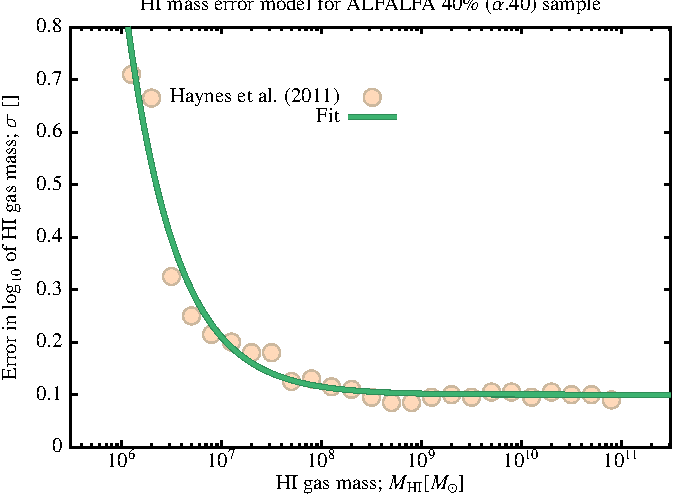
\includegraphics[width=85mm,trim=0mm 0mm 0mm 4mm,clip]{Plots/DataAnalysis/alfalfaHIMassErrorModel.pdf}
 \caption{The observational random error in galaxy HI mass as a function of HI mass for the ALFALFA survey. Points show the errors reported by \protect\cite{haynes_arecibo_2011}, while the line shows a simple functional form fit to these errors.}
 \end{center}
 \label{fig:ALFALFAErrorModel}
\end{figure}

Additionally, HI mass estimates can be affected by HI self-absorption for highly inclined galaxies. \cite[][see also \protect\citealt{zwaan_hipass_2005}]{zwaan_h_1997} estimate that this effect would lead to a mean underestimation of HI masses by a factor $1.1$ for a randomly oriented galaxy sample. Therefore, a value of $-0.0414$ for the systematic parameter {\normalfont \ttfamily [alfalfaHiMassFunctionZ0.00MassSystematic0]} is recommended.


\chapter{Plotting Support}\index{plotting}

\section{Plotting with {\normalfont \scshape Gnuplot}}

While \glc\ data can, of course, be plotted using whatever method you choose, two Perl modules are provided that we find useful for plotting \glc\ data. These are intended for use with \href{http://www.gnuplot.info/}{\normalfont \scshape GnuPlot} and with datasets stored as \href{http://pdl.perl.org/}{\normalfont \ttfamily PDL} variables. The first module, {\normalfont \ttfamily GnuPlot::PrettyPlots} plots lines and points with two color style (typically a lighter interior color and a darker border) with support for errorbars and limits (show as arrows) on points. The second, {\normalfont \ttfamily GnuPlot::LaTeX} provides a convenient way to process output from {\normalfont \scshape GnuPlot}'s {\normalfont \ttfamily epslatex} terminal into PDF files (suitable for inclusion in documents), PNG images with transparent backgrounds or \href{http://www.openoffice.org/}{OpenOffice} \href{http://www.wikimedia.org/wikipedia/en/wiki/OpenDocument}{ODG} files (suitable for inclusion into presentations\footnote{If you create an OpenOffice ODG file it's recommended that you covert it to a Metafile within OpenOffice before putting it into a presentation---this seems to prevent a bug which occasionally causes an element of the plot to be lost during saving\ldots}).

A typical use of these packages would look as follows:
\begin{verbatim}
use lib "./perl";
use PDL;
use GnuPlot::LaTeX;
use GnuPlot::PrettyPlots;

$outputFile = "myImage";
open($gnuPlot,"|gnuplot");
print $gnuPlot "set terminal epslatex color colortext lw 2 solid 7\n";
print $gnuPlot "set output '".$outputFile.".eps'\n";
print $gnuPlot "set xlabel '\$x-axis label\$'\n";
print $gnuPlot "set ylabel '\$y-axis label\$'\n";
print $gnuPlot "set lmargin screen 0.15\n";
print $gnuPlot "set rmargin screen 0.95\n";
print $gnuPlot "set bmargin screen 0.15\n";
print $gnuPlot "set tmargin screen 0.95\n";
print $gnuPlot "set key spacing 1.2\n";
print $gnuPlot "set key at screen 0.4,0.8\n";
print $gnuPlot "set key left bottom\n";
print $gnuPlot "set xrange [0.0:6.0]\n";
print $gnuPlot "set yrange [0.0:1.0]\n";
print $gnuPlot "set pointsize 2.0\n";
&PrettyPlots::Prepare_Dataset(\$plot,
			      $x1Data, $y1Data,
                              title => "First dataset",
                              style => line,
                              linePattern => 0,
                              weight => [7,3],
			      color => $PrettyPlots::colorPairs{'lightGoldenrod'}
                             );
&PrettyPlots::Prepare_Dataset(\$plot,
			      $x2Data, $y2Data,
			      errorDown => $errorDown,
			      errorUp   => $errorUp,
                              title => "Galacticus",
			      style => point,
                              symbol => [6,7],
                              weight => [5,3],
			      color => $PrettyPlots::colorPairs{'redYellow'}
                             );
&PrettyPlots::Plot_Datasets($gnuPlot,\$plot);
close($gnuPlot);
&LaTeX::GnuPlot2PNG($outputFile.".eps", backgroundColor => "#000080", margin => 1);
\end{verbatim}

The process begins by opening a pipe to {\normalfont \scshape GnuPlot} and specifying the {\normalfont \ttfamily epslatex} terminal along with {\normalfont \ttfamily color} and {\normalfont \ttfamily colortext} options, any line weight preferences and the output EPS file. This is followed by commands to set up the plot, including labels, ranges etc. Note that you \emph{must} specify margins manually\footnote{The {\normalfont \ttfamily GnuPlot::PrettyPlots} module works by generating multiple layers of plotting which are overlaid. Axes are only drawn for the first layer. If you do not specify margins manually, they will be computed automatically for each layer and so will not match up between all layers. This will result in data being plotted incorrectly.}. Following this are calls to {\normalfont \ttfamily \&PrettyPlots::Prepare\_Dataset} which prepares instructions for plotting of a single dataset. The first argument is a reference to a structure which will store the instructions, while the second and third arguments are PDLs containing the $x$ and $y$ data to be plotted. Following this are multiple options as follows:
\begin{description}
\item[{\normalfont \ttfamily title}] Gives the title of the dataset for inclusion in the plot key;
\item[{\normalfont \ttfamily style}] Specifies how the dataset should be drawn: either {\normalfont \ttfamily line}, {\normalfont \ttfamily point}, {\normalfont \ttfamily boxes}, or {\normalfont \ttfamily filledCurve};
\item{{\normalfont \ttfamily linePattern}} Specifies the line pattern (as defined for {\normalfont \scshape GnuPlot}'s {\normalfont \ttfamily lt} option) to use;
\item[{\normalfont \ttfamily symbol}] A two element list giving the symbol indices that should be used to plot the border and inner parts of each point respectively;
\item[{\normalfont \ttfamily weight}] A two element list giving the line weights to be used for border and inner parts of each point/line respectively;
\item[{\normalfont \ttfamily color}] A two element list giving the color of border and inner parts of each point/line respectively. Colors should be specified as {\normalfont \ttfamily \#RRGGBB} in hexadecimal. Several suitable color pairs and sequences of pairs are defined in the {\normalfont \ttfamily GnuPlot::PrettyPlots} module;
\item[{\normalfont \ttfamily pointSize}] Specifies the size of the points to be used;
\item[{\normalfont \ttfamily errorNNN}] Gives a PDL containing sizes of errors to be plotted on points in the up, down, left and right directions. A zero value will cause the error bar to be omitted, while a negative value will cause an arrow to be drawn with a length equal to the absolute value of the specified value;
\item[{\normalfont \ttfamily filledCurve}] If the {\normalfont \ttfamily filledCurve} style is used, this option specifies the type of filled curve ({\normalfont \ttfamily closed}, {\normalfont \ttfamily x1}, {\normalfont \ttfamily x2}, etc.---see the {\normalfont \scshape GnuPlot} {\normalfont \ttfamily help filledcurve} text for complete options). The default is {\normalfont \ttfamily closed};
\item[{\normalfont \ttfamily y2}] If the {\normalfont \ttfamily filledCurve} style is used along with the {\normalfont \ttfamily filledCurve}$=${\normalfont \ttfamily closed} option, this option is used to specify a second PDL of $y$-axis values. The region between this curve and the usual $y$-axis curve will be filled.
\end{description}
Once all datasets have been prepared, the call to {\normalfont \ttfamily \&PrettyPlots::Plot\_Datasets} will generate the EPS and \LaTeX\ files necessary to make the plot. This resulting plot can be converted to PDF, PNG or ODG form by calling {\normalfont \ttfamily \&LaTeX::GnuPlot2PDF}, {\normalfont \ttfamily \&LaTeX::GnuPlot2PNG} or {\normalfont \ttfamily \&LaTeX::GnuPlot2ODG} respectively. The EPS file will be replaced with the appropriate file. The {\normalfont \ttfamily \&LaTeX::GnuPlot2PNG} routine accepts an optional {\normalfont \ttfamily backgroundColor} argument in {\normalfont \ttfamily \#RRGGBB} format. If present, this color will be used to set the background color of the plot (otherwise white is assumed). Although the background is made transparent in the PNG, setting the background color is important as antialiasing will make use of this background. Note that both PNG and ODG options will switch black axes and labels to white\footnote{This is just a presonal preference for plots displayed in presentations---other options could be added}. Finally, the {\normalfont \ttfamily \&LaTeX::GnuPlot2PNG} routine accepts an optional {\normalfont \ttfamily margin} argument which specifies the size of the margin (in pixels) to be left around the plot when cropping.

The ODG option requires that both \href{http://www.cityinthesky.co.uk/opensource/pdf2svg}{{\normalfont \ttfamily pdf2svg}} and \href{http://www.haumacher.de/svg-import/}{{svg2office}} be installed on your system ({\normalfont \ttfamily svg2office} should be located in {\normalfont \ttfamily /usr/local/bin}).

\section{Merger Tree Diagrams with {\normalfont \scshape dot}}\index{merger trees!graphing}

The {\normalfont \scshape dot} command, which is a part of \href{http://www.graphviz.org/}{{\normalfont \scshape GraphViz}}\index{graphviz@{\normalfont \scshape GraphViz}} is useful for creating diagrams of merger trees. \glc\ provides a function to output the structure of any merger tree in {\normalfont \scshape GraphViz} format. This function, \hyperlink{objects.merger_trees.dump.F90:merger_trees_dump:merger_tree_dump}{{\normalfont \ttfamily Merger\_Tree\_Dump}}, is provided by the \hyperlink{objects.merger_trees.dump.F90:merger_trees_dump:merger_tree_dump}{{\normalfont \ttfamily Merger\_Trees\_Dump}} module. Usage is as follows:
\begin{lstlisting}[escapechar=@,breaklines,prebreak=\&,postbreak=\&]
call Merger_Tree_Dump(                                    &
     &                index                             , &
     &                baseNode                          , &
     &                highlightNodes     =highlightNodes, &
     &                backgroundColor    ='white'       , &
     &                nodeColor          ='black'       , &
     &                highlightColor     ='black'       , &
     &                edgeColor          ='#DDDDDD'     , &
     &                nodeStyle          ='solid'       , &
     &                highlightStyle     ='filled'      , &
     &                edgeStyle          ='solid'       , &
     &                labelNodes         =.false.       , &
     &                scaleNodesByLogMass=.true.        , &
     &                edgeLengthsToTimes =.true.        , &
     &                path               ='/my/path'      &
     &               )
\end{lstlisting}
Here {\normalfont \ttfamily index} is the tree index (successive calls to \hyperlink{objects.merger_trees.dump.F90:merger_trees_dump:merger_tree_dump}{{\normalfont \ttfamily Merger\_Tree\_Dump}} with the same index will result in a sequence of output files---see below), and {\normalfont \ttfamily baseNode} is a pointer to the base node of the tree to be dumped. All other arguments are optional:
\begin{description}
 \item [{\normalfont \ttfamily highlightNodes}] A list of node IDs. All nodes listed will be highlighted in the diagram;
 \item [{\normalfont \ttfamily backgroundColor}] The color for the background of the diagram;
 \item [{\normalfont \ttfamily nodeColor}] The color used to draw nodes;
 \item [{\normalfont \ttfamily highlightColor}] The color used for highlighted nodes;
 \item [{\normalfont \ttfamily edgeColor}] The color of edges (lines joining nodes);
 \item [{\normalfont \ttfamily nodeStyle}] The style to use when drawing nodes;
 \item [{\normalfont \ttfamily highlightStyle}] The style to use when drawing highlighted nodes;
 \item [{\normalfont \ttfamily edgeStyle}] The style to use when drawing edges;
 \item [{\normalfont \ttfamily labelNodes}] Specifies whether or not nodes should be labelled (labels consist of the node ID followed by the redshift);
 \item [{\normalfont \ttfamily scaleNodesByLogMass}] If true, the size of nodes will be set to be proportional to the logarithm of the node mass;
 \item [{\normalfont \ttfamily edgeLengthsToTimes}] If true, the spacing between parent and child nodes will be proportional to the logarithmic time interval between them.
 \item [{\normalfont \ttfamily path}] If present, write tree dumps into this directory. Otherwise, the current directory will be used.
\end{description}
All colors and styles are character strings and can be in any format understood by {\normalfont \scshape dot}. The tree structure will be dumped to file named {\normalfont \ttfamily mergerTreeDump:$\langle$ID$\rangle$:$\langle$N$\rangle$.gv} where {\normalfont \ttfamily $\langle$ID$\rangle$} is the index of the tree and {\normalfont \ttfamily $\langle$N$\rangle$} increasing incrementally from $1$ each time the same tree is consecutively dumped. These files can be processed using {\normalfont \scshape dot}. For example
\begin{verbatim}
 dot -Tps mergerTreeDump:1:1.gv > tree.ps
\end{verbatim}
will create a tree diagram as the PostScript file {\normalfont \ttfamily tree.ps}.


\chapter{Tutorials}

This chapter contains step-by-step guides to performing common tasks with \glc.

\section{Running \glc\ on N-body Merger Trees}\label{sec:nBodyRun}\index{merger trees!N-body}\index{N-body!merger trees}

See \S\ref{main-sec:MergerTreeBuilder} for details of how to build merger tree files suitable for input into \glc. There are many options which control precisely how merger trees read from file should be handled. The following section provides guidance on the best choice of parameters.

\subsection{Setting Input Parameters}

To utilize merger trees from the file\footnote{The following assumes that merger trees will be read from a file following \protect\glc's standard HDF5 format which is described in Appendix~\protect\ref{main-sec:MergerTreeFileFormat}.} that you created in a \glc\ run it's necessary to set two parameters in the input parameter file that you will use for the run:
\begin{verbatim}
  <!-- Specify that merger trees are to be read from file, and give the name of the file to read -->
  <mergerTreeConstructMethod value="read"             />
  <mergerTreeReadFileName    value="myNBodyTrees.hdf5"/>
\end{verbatim}
The first of these {\normalfont \ttfamily [mergerTreeConstructMethod]}$=${\normalfont \ttfamily read} tells \glc\ that merger trees will be constructed by reading them from a file. The second, {\normalfont \ttfamily [mergerTreeReadFileName]}, gives the name of the file from which to read the trees.

In order to choose sensible settings for the various parameters that control merger trees read from file, it is recommended that you read through each of the items below and follow the guidance given.

{\normalfont \bfseries Cosmology:} In addition to specifying that trees should be read from a file, it's also important to ensure that the values of cosmological parameters in \glc\ match those in the merger tree file. (If they don't match, \glc\ will stop with an error message unless you set {\normalfont \ttfamily [mergerTreeReadMismatchIsFatal]}$=${\normalfont \ttfamily false} in which case you'll just be warned about any mismatch.) In our case of using merger trees from the Millennium Simulation, the correct cosmological parameter values can be set as follows:
\begin{verbatim}
  <!-- Use Millennium Simulation cosmology. -->
  <cosmologyParametersMethod value="simple"/>
   <HubbleConstant  value="73.0"  />
   <OmegaMatter     value="0.25"  />
   <OmegaDarkEnergy value="0.75"  />
   <OmegaBaryon     value="0.0455"/>
  </cosmologyParametersMethod>
  <cosmologicalMassVarianceMethod value="filteredPower">
    <sigma_8 value="0.900"/>
  </cosmologicalMassVarianceMethod>
  <powerSpectrumPrimordialMethod value="powerLaw">
    <index               value="1.000"/>
    <wavenumberReference value="1.000"/>
    <running              value="0.000"/>
  </powerSpectrumPrimordialMethod>
\end{verbatim}

{\normalfont \bfseries Existance at Final Time:} Normally, \glc\ assumes that all merger trees will exist (i.e. have at least one node present) at the final output time. This may not be true of trees extracted from an N-body simulation---in this case \glc\ can be informed of this fact by setting:
\begin{verbatim}
  <allTreesExistAtFinalTime value="false"/>
\end{verbatim}

{\normalfont \bfseries Snapping Nodes to Snapshots:} N-body merger trees are often built from ``snapshots'' of the simulation, i.e. all of the nodes exist at a set of discrete times. Often we want to output nodes at precisely these output times. In such cases it is useful to set:
\begin{verbatim}
  <mergerTreeReadOutputTimeSnapTolerance value="1.0d-3"/>
\end{verbatim}
which ensures that the times of nodes are adjusted to lie at precisely the output time if that time is within the specified relative tolerance (this avoids any small differences between node times and output times that can arises due to rounding errors when converting from redshifts to times and vice-versa).

{\normalfont \bfseries Missing Hosts:} \glc\ expects to find each \gls{node}'s host \gls{node} present in a merger tree \gls{forest}. If a \gls{node}'s host is not found this is cause for a fatal error to be issued, since it is impossible to correctly construct and evolve the corresponding \gls{forest}. If you absolutely want to run a \gls{forest} for which one or more host \glspl{node} are missing, you can allow this by setting {\normalfont \ttfamily [mergerTreeReadMissingHostsAreFatal]}$=${\normalfont \ttfamily false}---in this case missing host \glspl{node} trigger a warning only and \glspl{node} without a host are forced to become isolated \glspl{node}. This will lead to incorrect tree evolution however, so the recommended setting is:
\begin{verbatim}
<mergerTreeReadMissingHostsAreFatal value="true"/>
\end{verbatim}

{\normalfont \bfseries Branch Jumps and Subhalo Promotions:} If your merger trees contain subhalos they will most likely exhibit two specific behaviors\footnote{These two behaviors are called out as they specifically \emph{do not} occur in merger trees created using Press-Schechter-based algorithms for example.}: i) \glspl{node} which are subhalos in one timestep may become non-subhalos (isolated halos) in a subsequent timestep (``subhalo promotion''), and ii) \glspl{node} which are subhalos in one branch of the tree may ``jump'' to another branch\footnote{That is, the subhalo's descendented is hosted by a \gls{node} other than the descendent of the subhalo's host.} of the tree becoming a subhalo there (``branch jumping''). These behaviors are fully supported by \glc\ and so we recommend the following settings:
\begin{verbatim}
<mergerTreeReadAllowSubhaloPromotions value="true"/>
<mergerTreeReadAllowBranchJumps       value="true"/>
\end{verbatim}
You may choose to disallow these behaviors by setting either of the above parameters to {\normalfont \ttfamily false}---for example if you wish to explore how your results would differ if subhalos were forced to remain subhalos forever in their original branch. Note that allowing subhalo promotion while not allowing branch jumping can lead to \glspl{deadlock} in merger tree evolution, so change these settings with caution.

Note that for trees which do not contain subhalos these two parameters are irrelevant.

{\normalfont \bfseries Subhalo Masses:} If your trees contain subhalos, the mass evolution of those subhalos can be preset in the satellite component of each \gls{node}. In this way, the subhalo mass in \glc\ will track that specified by the merger tree file. This requires the use of a satellite component which allows presetting of subhalo masses. Recommended settings are therefore:
\begin{verbatim}
<treeNodeMethodSatellite           value="preset"/>
<mergerTreeReadPresetSubhaloMasses value="true"  />
\end{verbatim}
If your trees do not contain subhalos, recommended settings are instead:
\begin{verbatim}
<treeNodeMethodSatellite           value="standard"/>
<mergerTreeReadPresetSubhaloMasses value="false"   />
\end{verbatim}

{\normalfont \bfseries Halo Positions/Velocities:} If your trees contain position and velocity information for halos, those positions and velocities can be preset in the position component of each \gls{node}. This requires the use of a position component which allows presetting of positions and velocities. Recommended settings are therefore:
\begin{verbatim}
<treeNodeMethodPosition        value="preset"/>
<mergerTreeReadPresetPositions value="true"  />
\end{verbatim}
If your trees do not contain position information recommended settings are:
\begin{verbatim}
<treeNodeMethodPosition        value="null" />
<mergerTreeReadPresetPositions value="false"/>
\end{verbatim}

{\normalfont \bfseries Subhalo Orbits:} If your trees contain position and velocity information they can be used to preset initial orbit information for subhalos. Note that it is not required that your trees contain subhalos for this orbit presetting to be performed---\glc\ can follow subhalo orbits even if subhalos are not included in the trees themselves. The following settings are recommended:
\begin{verbatim}
<mergerTreeReadPresetOrbits             value="true"/>
<mergerTreeReadPresetOrbitsSetAll       value="true"/>
<mergerTreeReadPresetOrbitsAssertAllSet value="true"/>
<mergerTreeReadPresetOrbitsBoundOnly    value="true"/>
\end{verbatim}
These options will cause an orbit to be preset for each subhalo based on the relative position and velocity of merging halos and assuming that the orbital energy and angular momentum are conserved between the time immediately prior to the merger and the time of virial radius crossing. If the computed orbit does not cross the virial radius of the larger halo or if the computed orbit is unbound, the above options cause an orbit to be preset by drawing orbital parameters at random from the chosen cosmological distribution (see \S\ref{main-sec:SatelliteVirialOrbits}).

{\normalfont \bfseries Subhalo Merging:} If your merger trees contain subhalo information, that information can be used to specify when, and with which other node, each subhalo merges. Specifically, a subhalo is assumed to merge at the time at which it is not the primary progenitor of its descendent halo---possibly with some other delay to be described below. Recommended settings are:
\begin{verbatim}
<mergerTreeReadPresetMergerTimes          value="true"             />
<mergerTreeReadPresetMergerNodes          value="true"             />
<mergerTreeReadSubresolutionMergingMethod value="boylanKolchin2008"/>
\end{verbatim}
The first two options cause subhalos to merge at the time described above, and with their descendent node. The final option accounts for the possibility that the subhalo should not actually merge immediately at this time. For example, in N-body simulations, the subhalo may have simply been lost due to limitations of resolution or halo finder algorithms. The final option specifies that some additional time until merging be added based on the subhalo merging timescale algorithm of \citeauthor{boylan-kolchin_dynamical_2008}~[\citeyear{boylan-kolchin_dynamical_2008}; see \S\ref{main-phys:satelliteMergingTimescales:satelliteMergingTimescalesBoylanKolchin2008}], and computed using the last known orbital properties of the subhalo.

{\normalfont \bfseries Halo Scale Radii:} If your merger trees contain information on halo scale radii or half-mass radii, these can be used to preset the scale radius of each \gls{node}. This requires the use of a dark matter profile component which allows presetting of scale length. Recommended settings are therefore:
\begin{verbatim}
<mergerTreeReadPresetScaleRadii                     value="true"     />
<mergerTreeReadPresetScaleRadiiFailureIsFatal       value="true"     />
<mergerTreeReadPresetScaleRadiiConcentrationMinimum value="3"        />
<mergerTreeReadPresetScaleRadiiConcentrationMaximum value="60"       />
<mergerTreeReadPresetScaleRadiiMinimumMass          value="see below"/>
\end{verbatim}
Minimum and maximum concentrations are specified---these are used to restrict the range of scale radii that are allowed for a given halo. If scale radii are to be determined based on half-mass radii given in the merger tree file, and if the computed scale radius does not result in a concentration between these limits, then a fatal error is issued.

Finally, you can set a minimum halo mass via the {\normalfont \ttfamily [mergerTreeReadPresetScaleRadiiMinimumMass]} parameter below which the scale radii or half-mass radii in your file should be considered not reliable. For halos below this mass, scale radii will instead be assigned via the selected dark matter halo concentration method (see \S\ref{main-sec:DarkMatterProfileConcentration}).

{\normalfont \bfseries Halo Angular Momenta:} If your merger trees contain spin or angular momentum information these can be preset for each node. Recommended settings are:
\begin{verbatim}
<treeNodeMethodSpin                  value="preset"/>
<mergerTreeReadPresetSpins           value="true"  />
<mergerTreeReadPresetUnphysicalSpins value="true"  />
\end{verbatim}
The last of these options causes any halos for which the spin given in the merger tree file is non-positive to be assigned a spin at random instead, drawn from the specified cosmological distribution (see \S\ref{main-sec:SpinParameterDistribution}).

If subhalo masses are not included in their host halo masses in your merger tree file, you should specify how the angular momenta of subhalos should be accounted for when adding their mass to their host halo. If positions and 3D angular momenta are available in your merger tree file, the recommended setting is:
\begin{verbatim}
<mergerTreeReadSubhaloAngularMomentaMethod value="summation"/>
\end{verbatim}
If this information is not present 
\begin{verbatim}
<mergerTreeReadSubhaloAngularMomentaMethod value="scale"    />
\end{verbatim}
should be used instead.

If your merger tree file contains 3D spin or angular momentum information, you can choose to make that information available within \glc\ be using the settings:
\begin{verbatim}
<treeNodeMethodSpin          value="preset3D"/>
<mergerTreeReadPresetSpins3D value="true"    />
\end{verbatim}

{\normalfont \bfseries Subhalo Indices:} If your merger trees contain subhalos, you can tell \glc\ to keep track of the indices of subhalos by setting:
\begin{verbatim}
<treeNodeMethodSatellite            value="preset"/>
<mergerTreeReadPresetSubhaloIndices value="true"  />
\end{verbatim}
The \glc\ output file will then contain {\normalfont \ttfamily satelliteNodeIndex} datasets which list the index (as given in the merger tree file) for all subhalos and halos. Without specifying this presetting, the index of subhalos is frozen at the index of the halo immediately prior to it becomming a subhalo.

The remainder of this section gives more detail about many of the parameters described above and how they affect handling of merger trees read from file. Further parameters can be set to control what information from the stored trees will be used in \glc. Examples are given below.

\subsection{Further Details}

Further details of the effects of the many parameters controlling merger trees read from file are given below.

\subsubsection{Node Positions}

If position and velocity information for tree nodes is available within the merger tree file then \glc\ can be instructed to use this information by using the ``preset'' method for tree node positions and telling the merger tree construction method to preset node positions as follows:
\begin{verbatim}
  <!-- Use merger tree node positions -->
  <treeNodeMethodPosition        value="preset"/>
  <mergerTreeReadPresetPositions value="true"  />
\end{verbatim}
If position information is unavailable, the ``null'' position method can be selected and the merger tree construction method instructed not to preset positions as follows:
\begin{verbatim}
  <!-- Do not use merger tree node positions -->
  <treeNodeMethodPosition        value="null" />
  <mergerTreeReadPresetPositions value="false"/>
\end{verbatim}

\subsubsection{Virial Orbits}\index{orbits!virial}\index{orbits!setting}\index{orbits!N-body}

If position and velocity information for tree nodes is available within the merger tree file then \glc\ can be instructed to use this information to estimate the orbit of each subhalo at the point at which it crosses the virial radius of its host halo. This ``virial orbit'' may then be used by, for example, calculations of merging timescales.
\begin{verbatim}
  <!-- Use merger tree node positions to compute orbits at the virial radius -->
  <mergerTreeReadPresetOrbits             value="true"/>
  <mergerTreeReadPresetOrbitsBoundOnly    value="true"/>
  <mergerTreeReadPresetOrbitsSetAll       value="true"/>
  <mergerTreeReadPresetOrbitsAssertAllSet value="true"/>
\end{verbatim}
Typically, a merging halo is not seen at precisely the time at which it crosses the virial radius of its host (due to the fact that N-body simulations are output at discretely spaced timesteps). Therefore, \glc\ computes the orbit at the time just prior to merging and assumes that the orbital parameters (energy and angular momentum) remain fixed to propagate the orbit to the virial radius of the host. The second parameter in the above example, {\normalfont \ttfamily [mergerTreeReadPresetOrbitsBoundOnly]}, specifies whether or not only bound orbits should be set. Some calculations (e.g. of subhalo merging times) assume bound orbits and may fail if given an unbound orbit. Setting this option to {\normalfont \ttfamily true} causes only bound orbits to be preset---unbound orbits are ignored. Note that some orbits cannot be propagated to the virial radius (i.e. their pericenter is larger than the virial radius). The {\normalfont \ttfamily [mergerTreeReadPresetOrbitsSetAll]} option, if true, will cause such orbits to be assigned randomly using the selected {\normalfont \ttfamily [virialOrbitsMethod]}, such that all orbits are assigned. The {\normalfont \ttfamily [mergerTreeReadPresetOrbitsAssertAllSet]} option requires that all orbits be set---if {\normalfont \ttfamily [mergerTreeReadPresetOrbitsSetAll]}$=${\normalfont \ttfamily false} and {\normalfont \ttfamily [mergerTreeReadPresetOrbitsAssertAllSet]}$=${\normalfont \ttfamily true} then \glc\ will exit with an error message if any orbit cannot be set.

If the satellite component additionally permits setting of the satellite position and velocity, these properties will also be assigned based on the relative position and velocity of the satellite and host halos.

\subsubsection{Merging Times and Targets}

The times at which subhalos merge with their host halo can be determined directly from the merger tree file if subhalo information is included in that file. Merging is assumed to occur when the subhalo no longer has a distinct descendent (i.e. it descends into a non-subhalo). If merging times are to be computed in this way set
\begin{verbatim}
  <treeNodeMethodSatellite         value="preset"/>
  <mergerTreeReadPresetMergerTimes value="true"  />
\end{verbatim}
which select a satellite orbit method that allows merger times to be present and tell the merger tree construction method to preset those merger times respectively. If merger times are not to be computed in this way then instead set, for example,
\begin{verbatim}
  <treeNodeMethodSatellite         value="standard" />
  <mergerTreeReadPresetMergerNodes value="false"    />
  <satelliteMergingMethod          value="Jiang2008"/>
\end{verbatim}
which selects a standard satellite orbit method, prevents attempts to preset the merger times and selects the {\normalfont \ttfamily Jiang2008} method for computing merger times instead.

In addition to setting the times of merger events, it is possible to set the target node with which a merging node should merge. By default, \glc\ will assume that all merging occurs with the non-subhalo host node in which a subhalo is located. This may not be the desired behavior when using N-body merger trees. For example, such trees may indicate that a subhalo merges with another subhalo. Setting
\begin{verbatim}
  <mergerTreeReadPresetMergerNodes value="true"/>
\end{verbatim}
will cause the target node with which each merger should occur to be determined from the merger tree structure and preset for use in \glc.

It is possible to add a delay between the last time at which a subhalo was seen in a simulation and the time at which it is considered to merge. This functionality is motivated by the consideration that a subhalo vanishing from a simulation may be simply due to it dropping below resolution rather than it actually having undergone a merger. The parameter {\normalfont \ttfamily [mergerTreeReadSubresolutionMergingMethod]} can be used to select a satellite merging timescale method (see \S\ref{main-sec:SatelliteMergingTimescales}) to use in this case. (It is set by default to ``{\normalfont \ttfamily null}'' such that no delay before merging occurs.) The orbit of the subhalo around its parent at the last time it is present in the merger tree is passed to this method and used to estimate a time until merging. This delay is added to the time at which the subhalo merges and, if merge target nodes are being set, the target node is updated accordingly.

\subsubsection{Subhalo Indices}

The indices of subhalos are usually frozen at the index of the halo just prior to becoming a subhalo. The index of the corresponding halo in the original tree (as read from file) can be tracked as follows:
\begin{verbatim}
  <treeNodeMethodSatellite            value="preset"/>
  <mergerTreeReadPresetSubhaloIndices value="true"  />
\end{verbatim}
to first select the ``preset'' satellite orbit method (which allows subhalo indices to be preset) and, second, to instruct the merger tree construction algorithm to preset those indices. The index will then be available in output as {\normalfont \ttfamily satelliteNodeIndex}.

\subsubsection{Subhalo Masses}

The masses of subhalos (specifically their time evolution after they become subhalos) can be set using the values stored in the merger tree file (if available). To set subhalo masses in this way use
\begin{verbatim}
  <treeNodeMethodSatellite           value="preset"/>
  <mergerTreeReadPresetSubhaloMasses value="true"  />
\end{verbatim}
to first select the ``preset'' satellite orbit method (which allows subhalo masses to be preset) and, second, to instruct the merger tree construction algorithm to preset those masses.

\subsubsection{Node Spins}

If information on the angular momenta of nodes is available in the merger tree file, this can be used to preset the value of the spin parameter in each node\footnote{Before doing this, it is important to be sure that the angular momenta of the nodes are reliable. For example, in low mass nodes extracted from an N-body simulation resolution effect may limit the accuracy of the measured angular momentum.} by setting:

\begin{verbatim}
  <mergerTreeReadPresetSpins value="true"/>
\end{verbatim}

The spin parameter is set using the spin of each node if available, or otherwise using the angular momentum of each node stored in the merger tree file using:
\begin{equation}
 \lambda = {|\mathbf{J}| |E|^{1/2} \over \mathrm{G} M^{5/2}}
\end{equation}
where $|\mathbf{J}|$ is the magnitude of the node's angular momentum, $M$ is the node's mass and $E$ is its energy. Additionally, by setting:

\begin{verbatim}
  <mergerTreeReadPresetSpins3D value="true"/>
\end{verbatim}
the spin vector of each node will be set (assuming that the vector spin or angular momenta of nodes are available in the merger tree file) using:
\begin{equation}
 \mathbf{\lambda} = {\mathbf{J} |E|^{1/2} \over \mathrm{G} M^{5/2}}.
\end{equation}

If spins could not be determined for some halos the spin (or angular momentum) should be set to zero in the merger tree file, and the parameter {\normalfont \ttfamily [mergerTreeReadPresetUnphysicalSpins]} set to {\normalfont \ttfamily true}. \glc\ will then assign a spin to such halos by sampling from the selected spin distribution (see \S\ref{main-sec:SpinParameterDistribution}). 

\subsubsection{Node Scale Radii}

If information on the half-mass or scale radii of nodes is available in the merger tree file, it can be used to preset the value of the dark matter halo scale radius in each node by setting:

\begin{verbatim}
  <mergerTreeReadPresetScaleRadii value="true"/>
\end{verbatim}

Before doing this, it is important to be sure that the half-mass or scale radii of the nodes are reliable. For example, in low mass nodes extracted from an N-body simulation resolution effect may limit the accuracy of the measured half-mass or scale radius. In such cases, use the {\normalfont \ttfamily [mergerTreeReadPresetScaleRadiiMinimumMass]} parameter to specify the lowest mass halos for which the scale radii should be preset---lower mass halos will be assigned a scale radius using the method specified by the {\normalfont \ttfamily [mergerTreeReadConcentrationFallbackMethod]} parameter (which will default to the value of {\normalfont \ttfamily [darkMatterConcentrationMethod]}; see \S\ref{main-sec:DarkMatterProfileConcentration}). It is also possible to specify minimum and maximum allowed concentrations when computing the scale radius from the half mass radius using the {\normalfont \ttfamily [mergerTreeReadPresetScaleRadiiConcentrationMinimum]} and {\normalfont \ttfamily [mergerTreeReadPresetScaleRadiiConcentrationMaximum]} parameters. If matching the half mass radius would require a concentration outside of this range, \glc\ will abort unless {\normalfont \ttfamily [mergerTreeReadPresetScaleRadiiFailureIsFatal]}$=${\normalfont \ttfamily false}, in which case it will instead silently use the fallback concentration method described above.

If only half-mass radii are available, the scale radius is set by using a root finding algorithm to ensure that half of the total halo mass is enclosed within the specified half-mass radius.

\subsubsection{Miscellaneous N-body Properties}

Several miscellaneous properties often available from N-body merger trees can also be preset by setting the following parameters to {\normalfont \ttfamily true}:
\begin{description}
\item[{mergerTreeReadPresetParticleCounts}] Sets the number of particles in each halo (requires the {\normalfont \ttfamily particleCount} dataset to be present in the merger tree file);
\item[{mergerTreeReadPresetVelocityMaxima}] Sets the maxima of halo rotation curves (requires the {\normalfont \ttfamily velocityMaximum} dataset to be present in the merger tree file);
\item[{mergerTreeReadPresetVelocityDispersions}] Sets the velocity dispersion of halos (requires the {\normalfont \ttfamily velocityDispersion} dataset to be present in the merger tree file).
\end{description}

\subsubsection{Subhalo Promotion}\label{sec:Tutorial:NbodyTrees:SubhaloPromotion}

A subhalo may, at a later time, become an isolated halo once again. \glc\ allows you to control whether such behavior is allowed, or should be prohibited. To allow such ``subhalo promotion'', set:
\begin{verbatim}
<mergerTreeReadAllowSubhaloPromotions value="true"/>
\end{verbatim}
If you choose to inhibit this behavior by setting the above parameter to false, a halo that becomes a subhalo will remain a subhalo forever thereafter. Note that the isolated halo to which it would have been promoted will still exist, and may therefore form its own galaxy. This can result in double counting of mass, and so inhibiting subhalo promotion is not recommended.

\subsubsection{``Fly-by'' Halos}\label{sec:Tutorial:NbodyTrees:BranchJump}

In some cases, a halo that is part of one tree can later become part of another tree. This can happen in so-called ``fly-by'' encounters where a halo may briefly become a subhalo in a halo in tree A then leave that halo and become a subhalo in tree B.

The correct way to handle this issue is to combine trees A and B into a single tree (which will now have multiple base nodes). \glc\ will then process these two trees simultaneously, correctly handling the fly-by, and outputting the trees as two separate trees.

If for some reason this is not possible or desired, the fly-by problem will normally cause \glc\ to complain that the host halo of a node cannot be found (since it exists in a different tree). This problem can be avoided by setting:
\begin{verbatim}
  <mergerTreeReadMissingHostsAreFatal value="false"/>
\end{verbatim}
In this case, nodes with missing hosts are simply treated as being isolated halos. This will avoid an error condition, but is not a physically correct way to handle such cases, so use with caution.

\subsection{Using Particles to Track Unresolved Subhalos}

In N-body simulations it is possible that a subhalo can become ``lost'' from the simulation (i.e. can no longer be identified by a halo finder due to resolution issues) before it has actually merged with the central galaxy or been completely tidally destroyed. In such cases it is useful to be able to assign a position to the subhalo at later times. A common approach to assigning a position (and velocity) is to use that of the most bound particle in the subhalo at the last time it was identified. \glc\ allows for particle tracking in this way through the addition of particle information to the merger tree file.

To add particle tracking data to a merger tree file, follow these steps:
\begin{enumerate}
\item Identify all subhalos which are lost from the simulation prior to the final timestep;
\item Determine the index of the most bound particle in each such subhalo in the last timestep in which it was identified;
\item For each subhalo, extract the redshift, position, and velocity of that particle (which is usally trivial to do once its index is known) at each subsequent timestep in the simulation;
\item Write these data (along with the particle index) to the {\normalfont \ttfamily particles} group in the merger tree file as described in \S\ref{main-sec:MergerTreeFormatDescription:Particles};
\item Add two datasets to the {\normalfont \ttfamily forestHalos} group:
  \begin{enumerate}
  \item {\normalfont \ttfamily particleIndexStart} which should indicate the index in the datasets in the {\normalfont \ttfamily particles} group at which the data for each halo begins (or $-1$ if no particle data is included for the halo);
  \item {\normalfont \ttfamily particleIndexCount} which should indicate the number of entries in the datasets in the {\normalfont \ttfamily particles} group for each halo (or $-0$ if no particle data is included for the halo).
  \end{enumerate}
\end{enumerate}

\subsection{Handling of Extremely Large Merger Tree Forests}\index{merger trees!large}\index{forests!large}

Halos can move between merger trees (see \S\ref{sec:Tutorial:NbodyTrees:SubhaloPromotion} and \S\ref{sec:Tutorial:NbodyTrees:BranchJump}), leading to the necessity of merger tree forests---interconnected groups of merger trees that \glc\ typically processes as a whole. These forests can become very large---in some cases so large that they do not fit within the available memory. \glc\ can handle such forests by splitting them into individual trees. Each tree is processed separately, and nodes are moved between trees as needed. If a tree needs a node from another tree before its evolution can continue, its state can be suspended to disk, and later re-read once the node it requires becomes available. In this way, very large forests can be processed without running out of memory (as trees are stored to disk while they are not being processed).

To cause forests to be split in this way, the following parameters should be set:
\begin{verbatim}
  <treeEvolveSuspendToRAM                   value="false"            />
  <treeEvolveSuspendPath                    value="/my/scratch/path/"/>
  <mergerTreeReadForestSizeMaximum          value="10000000"         />
  <mergerTreeReadSubresolutionMergingMethod value="infinite"         />
\end{verbatim}

Here, {\normalfont \ttfamily treeEvolveSuspendToRAM} specifies that merger trees should be suspended to disk (i.e. not to RAM which is the default), and {\normalfont \ttfamily treeEvolveSuspendPath} gives a path where the suspended trees can be written---typically scratch space local to the compute node where \glc\ is being run is a good option.
 
{\normalfont \ttfamily mergerTreeReadForestSizeMaximum} specifies the maximum number of nodes allowed in a forest before it will be split. A suitable number for this depends on the details of the available RAM, the number of threads sharing that RAM, and the characteristics of the \glc\ model being used (which will affect the memory required per node).
 
Finally, {\normalfont \ttfamily mergerTreeReadSubresolutionMergingMethod} is set to {\normalfont \ttfamily infinite} to prevent any merging (which is not supported for split forests at present, although it should be soon).

\subsection{Analyzing the Output}

\subsubsection{Positions and Velocities}

Components of the position of each node are output as {\normalfont \ttfamily positionX}, {\normalfont \ttfamily positionY} and {\normalfont \ttfamily positionZ} and can be accessed in the same way as other output properties from \glc\ (see \S\ref{sec:nodeDataGroup} and \S\ref{sec:perlModuleDataExtraction}).

\subsubsection{Subhalo Masses}

The current mass of subhalos is available via the {\normalfont \ttfamily nodeBoundMass} output dataset and can be accessed in the same way as other output properties from \glc\ (see \S\ref{sec:nodeDataGroup} and \S\ref{sec:perlModuleDataExtraction}). For non-subhalos this property is equal to the usual {\normalfont \ttfamily nodeMass} property.

\section{Generating Mock Catalogs with Lightcones from the Millennium Simulation}\index{lightcone}\index{Millennium Simulation}\index{mock catalog}

Suppose that you want to create a catalog of galaxies as would be found in a survey of an area of the sky out to some redshift. Such a ``mock catalog'' can be built by populating with galaxies all of the dark matter halos which happen to lie within the cone which that area makes as it is projected from the observer through the Universe.

Generating such a mock catalog using \glc\ involves first extracting the halos (and their merger trees) within this ``lightcone'' from a suitable N-body simulation, and then processing them through \glc. In this tutorial, we will specifically make use of the \href{http://gavo.mpa-garching.mpg.de/MyMillennium3/MyDB}{Millennium Simulation database} to provide the merger trees, but the same principles apply to any N-body simulation.

The script, {\normalfont \ttfamily scripts/aux/Millennium\_Lightcone\_Grab.pl} can be used to retrieve merger trees that intersect a given lightcone from the Millennium Database and to store them in \glc's format (see \S\ref{main-sec:MergerTreeFileFormat}). The script is used as follows:
\begin{verbatim}
scripts/aux/Millennium_Lightcone_Grab.pl <lightconeDirectory> <fieldSize> <maximumRedshift>
    --user <myUserName> --password <myPassword> --treesPerFile <treesPerFile>
\end{verbatim}
Here, {\normalfont \ttfamily \textless lightconeDirectory\textgreater} is the name of a (pre-existing) directory into which merger tree data will be stored, {\normalfont \ttfamily \textless fieldSize\textgreater} is the length (in degrees) of one side of the square field of view of the lightcone, {\normalfont \ttfamily \textless maximumRedshift\textgreater} is the highist redshift for which halos should be included in the catalog. The {\normalfont \ttfamily --user} and {\normalfont \ttfamily --password} options allow you to specify your username and password for accessing the Millennium Simulation database. Finally, the {\normalfont \ttfamily --treesPerFile} specifies how many merger trees should be stored in each file (the script will split the lightcone between many files---this is primarily so that each request sent to the Millennium Database server is not too large). If no value is specified a default of 200 trees per file will be used.

The script generates multiple SQL queries to the Millennium database in order to first find all halos which intersect the lightcone and second to retrieve the complete merger tree associated with each such halo. These merger trees are then stored in \glc's merger tree file format in files named {\normalfont \ttfamily Lightcone\_Trees\_AAA:BBB.hdf5} in the given {\normalfont \ttfamily \textless lightconeDirectory\textgreater}, where {\normalfont \ttfamily AAA} and {\normalfont \ttfamily BBB} are numbers giving the first and last trees in the file\footnote{Note that these are not the ID numbers of the trees, just a sequential count of all trees retrieved.}

Each of the merger tree files created can then be run through \glc\ in the usual way (see \S\ref{sec:nBodyRun}).  Outputs should be requested at every Millennium snapshot (up to the largest redshift to be considered), and the {\normalfont \ttfamily lightcone} filter should be used to cause only those galaxies which intersect the lightcone to be output---for example:
\begin{verbatim}
<!-- Set output redshifts to the snapshots in the milliMillennium. -->
<outputRedshifts value=
   "0.0000 0.0199 0.0414 0.0645 0.0893 0.1159 0.1444 0.1749 0.2075 0.2425
    0.2798 0.3197 0.3623 0.4079 0.4566 0.5086 0.5642 0.6236 0.6871 0.7550
    0.8277 0.9055 0.9887 1.0779 1.1734 1.2758 1.3857 1.5036 1.6303 1.7663
    1.9126 2.0700 2.2395 2.4220 2.6189 2.8312 3.0604 3.3081 3.5759 3.8657
    4.1795 4.5196 4.8884 5.2888 5.7239 6.1968"
/>

<!-- Add a lightcone filter with the required geometry -->
<mergerTreeOutput>
  <galacticFilterMethod value="lightcone"/>
</mergerTreeOutput>

<!-- Switch on output of lightcone data -->
<outputLightconeData value="true"/>

<!-- Prune away trees not appearing in the lightcone -->
<mergerTreeOperatorMethod value="pruneLightcone"/>

<!-- Specify lightcone geometry -->
<geometryLightconeMethod value="square">
  <origin value="0 0 0"/>
  <unitVector1 value=" 1 1  1"/>
  <unitVector2 value=" 0 1 -1"/>
  <unitVector3 value="-2 1  1"/>
  <lengthReplication value="500"/>
  <lengthHubbleExponent value="-1"/>
  <lengthUnitsInSI value="3.08567758135e22"/>
  <angularSize value="0.5"/>
  <timeEvolvesAlongLightcone value="true"/>
  <redshift value=
   "0.0000 0.0199 0.0414 0.0645 0.0893 0.1159 0.1444 0.1749 0.2075 0.2425
    0.2798 0.3197 0.3623 0.4079 0.4566 0.5086 0.5642 0.6236 0.6871 0.7550
    0.8277 0.9055 0.9887 1.0779 1.1734 1.2758 1.3857 1.5036 1.6303 1.7663
    1.9126 2.0700 2.2395 2.4220 2.6189 2.8312 3.0604 3.3081 3.5759 3.8657
    4.1795 4.5196 4.8884 5.2888 5.7239 6.1968"
  />
</geometryLightconeMethod>
\end{verbatim}
In the above {\normalfont \ttfamily [outputLightconeData]} causes lightcone coordinate information (i.e. the position and velocity of each galaxy in a coordinate system with axes aligned along the line of sight of the lightcone and parallel to the two edges of the square field of view, along with the redshift) to be output (see \S\ref{main-sec:OutputLightcone}), and {\normalfont \ttfamily [mergerTreeOperatorMethod]} is set to {\normalfont \ttfamily pruneLightcone} to cause any merger trees which have no nodes within the lightcone volume to be pruned away (as there is no need to process them). Finally, the {\normalfont \ttfamily geometryLightconeMethod} parameter describes the geometry of the lightcone to be used---see \S\ref{main-sec:methodsGeometryLightcone} for details.

\section{Using the Instantaneous Recycling Approximation}\index{recycling!instantaneous}\index{instantaneous recycling approximation}

Choosing {\normalfont \ttfamily [stellarPopulationPropertiesMethod]}$=${\normalfont \ttfamily instantaneous} will cause \glc\ to use the instantaneous recycling approximation for all calculations of stellar populations. The recyling rate and yield to use are set by the {\normalfont \ttfamily [imfNAMERecycledInstantaneous]} and {\normalfont \ttfamily [imfNAMEYieldInstantaneous]} parameters respectively, where {\normalfont \ttfamily NAME} is the name of the appropriate \gls{imf}.

Setting {\normalfont \ttfamily [stellarPopulationPropertiesMethod]}$=${\normalfont \ttfamily noninstantaneous} causes \glc\ to use a fully non-instantaneous, metal-depdendent calculation of recycling, metal production and \gls{sne} rates. However, it is possible to force this method to operate in the instantaneous recycling approximation limit (which can be useful for testing and comparison) by setting:
\begin{verbatim}
  <!-- Force the calculation of recycling, yields etc. to   -->
  <!-- be done assuming instantaneous recycling             -->
  <starFormationImfInstantaneousApproximation value="true"/>
  <!-- Set the mass of stars which should be used as the    -->
  <!-- dividing line between long-lived and instantaneously -->
  <!-- evolving in this approximation.                      -->
  <starFormationImfInstantaneousApproximationMassLongLived value="1.0"/>
  <!-- Set the effective age of populations to use in this -->
  <!-- approximation when computing SNe numbers.           -->
  <starFormationImfInstantaneousApproximationEffectiveAge value="13.8"/>
\end{verbatim}

\section{Computing Dust Attenuated Luminosities for All Galaxies}\label{sec:TutorialDustAttenuation}\index{dust!attenuation}

As described in \S\ref{sec:DerivedProperties}, dust-attenuated luminosities can be computed for galaxies using the calculations of \cite{ferrara_atlas_1999} (among other methods). A script is provided which will automatically perform this calculation for all filters, in all galaxies, at all output redshifts in a \glc\ output file and store the results (along with the assumed galaxy inclinations) back to the \gls{hdf5} file. The script is used as follows:
\begin{verbatim}
./scripts/analysis/dustExtinguish.pl <galacticusFileName>
\end{verbatim}

\section{Computing Dust Attenuation and Emission Using Galacticus+Grasil}\label{sec:TutorialGrasil}\index{dust!emission}\index{dust!attenutation}\index{Grasil@{\normalfont \scshape Grasil}}

\glc\ can interface with the \href{http://adlibitum.oat.ts.astro.it/silva/grasil/grasil.html}{\normalfont \scshape Grasil} code to compute the attenutation of starlight by dust, along with the re-emission of absorbed energy by that dust. To do this, it is necessary to store the entire star formation history of galaxies in a \glc\ model, as {\normalfont \scshape Grasil} uses this information to determine the attenuation of stellar populations as a function of their age.

Recording star formation histories is as simple as setting the {\normalfont \ttfamily [starFormationHistoriesMethod]} parameter to {\normalfont \ttfamily metallicitySplit}. This particular star formation history method stores the star formation in each galaxy as a function of time and metallicity, as required by {\normalfont \scshape Grasil}. The level of detail with which the star formation history is stored is controlled by several parameters:
\begin{description}
\item [{\normalfont \ttfamily starFormationHistoryTimeStep}] The timestep used in discretizing star formation histories.
\item [{\normalfont \ttfamily starFormationHistoryFineTimeStep}] The timestep to use in discretizing star formation histories just prior to output times. This should typically be smaller than {\normalfont \ttfamily [starFormationHistoryTimeStep]} to give improved resolution in the star formation history for recently formed stars.
\item [{\normalfont \ttfamily starFormationHistoryFineTime}] The period before each output for which the {\normalfont \ttfamily [starFormationHistoryFineTimeStep]} should be used.
\item [{\normalfont \ttfamily starFormationHistoryMetallicityCount}] The number of bins in metallicity to use when discretizing the star formation history.
\item [{\normalfont \ttfamily starFormationHistoryMetallicityMinimum}] The upper limit to the metallicity in the lowest metallicity bin (i.e. the lowest metallicity bin will extend from zero to this value).
\item [{\normalfont \ttfamily starFormationHistoryMetallicityMaximum}] The upper limit to the metallicity in the highest metallicity bin.
\end{description}
Default values set a timestep of 0.1~Gyr, with 0.01~Gyr timesteps for 0.1~Gyr before each output, along with 10 metallicity bins ranging from $10^{-4}Z_\odot$ to $10Z_\odot$. It is always recommended to check that these values result in a sufficiently well-resolved star formation history for your purposes.

When run with these parameter settings \glc\ will output an additional group to the output file called {\normalfont \ttfamily starFormationHistories}. This contains a hierarchically arranged set of datasets describing the star formation histories. The hierarchy extends through output number, and merger tree index. For example {\normalfont \ttfamily starFormationHistories/Output5/mergerTree3/} will contain the star formation history for merger tree 3 at output 5. This group will, in general, contain many datasets, e.g.
\begin{verbatim}
diskSFH7819       Dataset {11, 34}
diskTime7819      Dataset {34}
spheroidSFH7819   Dataset {11, 34}
spheroidTime7819  Dataset {34}
\end{verbatim}
In this case, datasets are present for both a disk and bulge component of node 7819. (If a node does not contain one of these components, the corresponding dataset will be missing.) The ``{\normalfont \ttfamily Time}'' datasets give the times at which the star formation history is stored, while the ``{\normalfont \ttfamily SFH}'' datasets give the mass of stars formed in each time/metallicity bin. (The metallicities themselves are available in the {\normalfont \ttfamily starFormationHistories/metallicities} dataset.)

Properties of the {\normalfont \scshape Grasil} \gls{sed} can now be accessed using the {\normalfont \ttfamily Galacticus::Grasil} module (see \S\ref{sec:Grasil}). When such properties are requested, {\normalfont \scshape Grasil} will be automatically run on each selected galaxy, the \gls{sed} computed and stored to the \glc\ file\footnote{{\normalfont \scshape Grasil} \glspl{sed} are stored in the {\normalfont \ttfamily grasilSEDs} group in a hierarchy of output, merger tree, and node groups, as for the star formation histories. Within each node group three datasets are stored, giving the {\normalfont \ttfamily wavelength}, {\normalfont \ttfamily inclination}, and {\normalfont \ttfamily SED} of the galaxy.}, and the relevant fluxes computed. If necessary, {\normalfont \scshape Grasil} and its data files will be downloaded automatically. Multiple {\normalfont \scshape Grasil} models will be run simultaneously if multiple cores are available.

For example:
\begin{verbatim}
# Specify model.                                                                                                                 
my $galacticus;
$galacticus->{'file' } = "/galacticus.hdf5";
$galacticus->{'store'} = 0;
$galacticus->{'tree' } = "all";

# Specify Grasil options.                                                                                                        
$galacticus->{'grasilOptions'}->{'includePAHs'            } = 1;
$galacticus->{'grasilOptions'}->{'fluctuatingTemperatures'} = 1;
$galacticus->{'grasilOptions'}->{'wavelengthCount'        } = 1000;
$galacticus->{'grasilOptions'}->{'radialGridCount'        } = 30;
$galacticus->{'grasilOptions'}->{'recomputeSEDs'          } = 0;
$galacticus->{'grasilOptions'}->{'launchMethod'           } = "pbs";

# Read results from model.                                                                                                       
&HDF5::Select_Output($galacticus,2.0);
&HDF5::Get_Dataset  ($galacticus,
                           [
                            'grasilFlux850microns',
                            'grasilFlux250microns',
                            'grasilFlux350microns',
                            'grasilFlux500microns',
                            'grasilInfraredLuminosity'
                           ]
\end{verbatim}
The {\normalfont \ttfamily grasilOptions} block in the above controls the behavior of {\normalfont \scshape Grasil}. Here we've chosen to include calculations of \gls{pah} features, have accounted for fluctuating tempertures in small grains (both of which slow down the calculation but make it more accurate), have specified the number of wavelengths and the size of the radial grid used to model each galaxy. We have also specified that the \gls{sed} should not be recomputed---if {\normalfont \scshape Grasil} fluxes are requested in future for galaxies in this model, they will be computed from the stored {\normalfont \scshape Grasil} \gls{sed}. If you want to change the parameters of the {\normalfont \scshape Grasil} calculation then set the {\normalfont \ttfamily recomputeSED} option to 1 instead\footnote{Exercise caution when using this option. Recomputing SEDs requires deleting the old SED group. The HDF5 library currently does not clean up the space occupied by the datasets in this deleted group, so the file size can grow rapidly if you repeatedly recompute {\normalfont \scshape Grasil} SEDs.}.

Finally, the {\normalfont launchMethod} option specifies how {\normalfont \scshape Grasil} is to be run. Currently supported options are {\normalfont \ttfamily local} and {\normalfont \ttfamily pbs}. Selecting {\normalfont \ttfamily local} causes {\normalfont \scshape Grasil} to be run on the local machine. Multiple threads are launched automatically, up to one per available CPU core unless otherwise specified. Selecting {\normalfont \ttfamily pbs} causes {\normalfont \scshape Grasil} jobs to be submitted to  a PBS queue.

Fluxes are returned in units of Janskys, while the total infrared luminosity ({\normalfont \ttfamily grasilInfraredLuminosity}) is returned in units of Solar luminosities.

A simple plotting script is provided which illustrates how to access and use the {\normalfont \scshape Grasil} \glspl{sed} stored in \glc\ files. For example:
\begin{verbatim}
scripts/plotting/plotGrasilSpectrum.pl galacticus.hdf5 5 9 217 43.2 SED.pdf
\end{verbatim}
will plot the \gls{sed} of node 217, in merger tree 9, at output 5 from the {\normalfont \ttfamily galacticus.hdf5} file. The \gls{sed} will be shown for an inclination of $43.2^\circ$ and the plot will be written to {\normalfont \ttfamily SED.pdf}.

\section{Outputting Stellar Luminosities}\index{luminosities!stellar}\index{stellar!luminosities}\index{luminosities!galactic}\index{galaxy!luminosities}

\glc\ can compute the stellar luminosity of galaxies in any required combination of filter, redshift, and frame. To cause luminosities to be computed add something such as the following to your input parameter file:
\begin{verbatim}
 <luminosityFilter   value="SDSS_r"  />
 <luminosityRedshift value="0.1"     />
 <luminosityType     value="observed"/>
\end{verbatim}
This would result in a dataset called {\normalfont \ttfamily diskLuminositiesStellar:SDSS\_r:observed:z0.1000} being output (along with a similar dataset for the spheroid component), corresponding to the luminosity in the SDSS r-band filter, as observed at $z=0.1$. To get the same filter but in the rest-frame of the galaxy, change the {\normalfont \ttfamily luminosityType} to ``{\normalfont \ttfamily rest}''. If instead of specifying a unique redshift you instead specify ``{\normalfont \ttfamily all}'' for a filter in the {\normalfont \ttfamily luminosityRedshift} element, then the filter will be replicated to all output redshifts.

Available filters can be found in the {\normalfont \ttfamily data/filters} folder. Additionally, it is possible to specify top-hat filters (which have unit transmission over a range of wavelengths) without the need to create a filter file for them. A filter named {\normalfont \ttfamily topHat\_L\_R} will be interpretted as a top-hat filter where {\normalfont \ttfamily L}$=\lambda$ is the central wavelength (in \AA ngstroms) and {\normalfont \ttfamily R}$=R$ is the resolution. A top-hat filter is constructed such that the transmission is unity between $\lambda_1$ and $\lambda_2$, and zero outside that range, and such that $\lambda_1\lambda_2=\lambda^2$, $\lambda_2-\lambda_1=\lambda/R$. Furthermore, a filter specified as {\normalfont \ttfamily topHat\_Llow\_Lhigh\_R} will be expanded into a set of contiguous top-hat filters with resolution {\normalfont \ttfamily R} spanning the wavelength range {\normalfont \ttfamily Llow} to {\normalfont \ttfamily Lhigh} with the first filter's lower wavelenght limit aligned with {\normalfont \ttfamily Llow} and continuing until the central wavelength of the filter is no longer below {\normalfont \ttfamily Lhigh}.

Luminosities are always output in units of the zero-point of the AB magnitude system, such that $-2.5\log_{10}L$ (where $L$ is the output luminosity) gives the AB absolute magnitude of the galaxy.

You can add additional luminosities by simply adding more entries in these parameter values. For example:
\begin{verbatim}
 <luminosityFilter   value="SDSS_r   SDSS_g"/>
 <luminosityRedshift value="0.1      0.3"   />
 <luminosityType     value="observed rest"  />
\end{verbatim}
would result in datasets {\normalfont \ttfamily diskLuminositiesStellar:SDSS\_r:observed:z0.1000} and {\normalfont \ttfamily diskLuminositiesStellar:SDSS\_g:rest:z0.3000}. 

\subsection{Postprocessing of Stellar Spectra}

Stellar luminosities are computed by convolving a library of simple stellar populations with the star formation history of each galaxy. \glc\ allows the spectra of those simple stellar populations to be postprocessed (after being read from file or internally generated for example) before they are utilized in the convolution integral. This postprocessing can modify the spectra in arbitrary ways that depend on wavelength, redshift, and age of stellar population. Furthermore, \glc\ allows you to chain together stellar spectra postprocessors into a set to allow multiple postprocessings to be applied. Furthermore again, you can define an arbitrary number of sets and apply different sets to different luminosities.

Typical uses of stellar spectra postprocessors include accounting for absorption of galaxy light by the intervening \gls{igm}, or capturing only the light from recent star formation\footnote{Perhaps so that additional dust extinction can be applied to the light of recently formed stars.}. A full list of the available postprocessors can be found in \S\ref{main-sec:StellarSpectraPostprocessing}.

If you don't specify a postprocessing set, the ``default'' set (consisting of the {\normalfont \ttfamily inoue2014} postprocessor; see \S\ref{main-phys:spectraPostprocessor:spectraPostprocessorInoue2014}) is applied to each luminosity calculation. To specify other postprocessing sets add the following to your parameter file:
\begin{verbatim}
 <luminosityPostprocessSet value="default recent unabsorbed recentUnabsorbed"/>
\end{verbatim}
where one set must be specified for each luminosity specified in the {\normalfont \ttfamily luminosityFilter} parameter. Note that set names can be reused in order to apply the same postprocessor set to multiple luminosities.

The chain of postprocessors to apply for each set is then specified as follows:
\begin{verbatim}
 <stellarPopulationSpectraPostprocessRecentMethods           value="inoue2014 recent"/>
 <stellarPopulationSpectraPostprocessUnabsorbedMethods       value="identity"        />
 <stellarPopulationSpectraPostprocessRecentUnabsorbedMethods value="recent"          />
\end{verbatim}
In this case we've constructed three new sets, in addition to the default set (which applies just the {\normalfont \ttfamily inoue2014} postprocessor). The {\normalfont \ttfamily recent} set applies both the {\normalfont \ttfamily inoue2014} \gls{igm} absorption postprocessor, followed by the {\normalfont \ttfamily recent} postprocessor to retain only recently emitted light. The {\normalfont \ttfamily unabsorbed} set ignores \gls{igm} absorption entirely---it does this by using the {\normalfont \ttfamily identity} postprocessor which leaves the spectrum unaffected. Finally, the {\normalfont \ttfamily recentUnabsorbed} set applies only the {\normalfont \ttfamily recent} filter while ignoring \gls{igm} absorption.

In this way it is relatively easy to extract multiple different measures of luminosity from a \glc\ model. For example, you could construct four postprocessor sets, each corresponding to one of the four different \gls{igm} absorption models ({\normalfont \ttfamily lycSuppress}, {\normalfont \ttfamily madau1995}, {\normalfont \ttfamily meiksin2006}, and {\normalfont \ttfamily inoue2014}) and apply these to the same luminosity filter to assess how luminosity depends on the \gls{igm} model used.

\subsection{Migrating Parameter Files to a New Version}\label{sec:MigrateParameters}\index{migration}\index{parameters}

The names and allowed values of parameters often change between versions of \glc. To permit easy and error-free migration between versions a script is provided to translate parameter files from earlier to later versions. To migrate a parameter file simply use:
\begin{verbatim}
scripts/aux/parametersMigrate.pl parameters.xml newParameters.xml
\end{verbatim}
By default, this script will translate from the previous to the current version of \glc. If your parameter file contains a {\normalfont \ttfamily version} element then this will be used to determine which version of \glc\ the parameter file was constructed for. The migration script will then migrate the parameter file through all intermediate versions to bring it into compliance with the current version. You can also specify input and output versions directly:
\begin{verbatim}
scripts/aux/parametersMigrate.pl parameters.xml newParameters.xml --inputVersion 0.9.0 --outputVersion 0.9.3
\end{verbatim}
will convert {\normalfont \ttfamily parameters.xml} from version 0.9.0 syntax to version 0.9.3 syntax.

\subsection{Computing Emission Lines}\label{sec:EmissionLineTutorial}\index{emission lines}\index{lines!emission}

\glc\ can compute emission line luminosities for galaxies. This calculation is based on the methodology of \cite{panuzzo_dust_2003}. Briefly, HII region models are constructed using {\normalfont \scshape Cloudy} for a variety of gas densities and metallicities, and HI, HeI, and OII ionizing luminosities. Emission line luminosities are then computed by interpolating in these tables based on the instantaneous properties of model galaxies.

To compute emission line luminosities it is therefore necessary to run \glc\ including the following rest-frame luminosity filters at each redshift of interest: {\normalfont \ttfamily Lyc}, {\normalfont \ttfamily HeliumContinuum}, {\normalfont \ttfamily OxygenContinuum}. This causes the ionizing luminosity for each three species to be computed and output. Emission line luminosities can then be found using \glc's data extraction modules (see \S\ref{sec:perlModuleDataExtraction}), by simply importing the {\normalfont \ttfamily Galacticus::EmissionLines} module. Emission line luminosites (in units of Solar luminosities) can then be accessed as named properties using names such as {\normalfont \ttfamily totalLineLuminosity:balmerAlpha6563:rest:z0.0000}, which will return the H$\alpha$ luminosity at $z=0$. Equivalent properties for disk and spheroid are provided (simply replace ``{\normalfont \ttfamily total}'' with ``{\normalfont \ttfamily disk}'' or ``{\normalfont \ttfamily spheroid}''). Currently available lines are:
\begin{itemize}
\item {\normalfont \ttfamily balmerAlpha6563}
\item {\normalfont \ttfamily balmerBeta4861}
\item {\normalfont \ttfamily oxygenII3726}
\item {\normalfont \ttfamily oxygenII3729}
\item {\normalfont \ttfamily oxygenIII4959}
\item {\normalfont \ttfamily oxygenIII5007}
\item {\normalfont \ttfamily nitrogenII6584}
\item {\normalfont \ttfamily sulfurII6731}
\item {\normalfont \ttfamily sulfurII6716}
\end{itemize}

Additionally, if a line is requested as {\normalfont \ttfamily totalLineLuminosity:balmerAlpha6563:<filterName>:rest:z0.0000} then the line luminosity is computed under the provided filter, and the luminosity is returned in units of \glspl{maggie} for easy conversion to magnitudes.

\subsection{Reionization Calculations}\label{sed:ReionziationTutorial}\index{reionization}

\glc\ can self-consistently solve for the evolution of the \gls{igm} as it becomes photoionized by light emitted by stars and AGN. To activate this calculation, include the following in your parameters file:
\begin{verbatim}
  <!-- IGM evolver -->
  <intergalacticMediumStateMethod  value="internal"/>
  <igmPropertiesCompute            value="true"    />
  <igmPropertiesTimeCountPerDecade value="10"      />
  
  <!-- Background radiation -->
  <backgroundRadiationCompute                  value="true"    />
  <radiationIntergalacticBackgroundMethod      value="internal"/>
  <backgroundRadiationWavelengthCountPerDecade value="50"      />
  <backgroundRadiationTimeCountPerDecade       value="10"      />

  <!-- Halo accretion options -->
  <accretionHaloMethod value="naozBarkana2007"/>
\end{verbatim}
The first block of parameters switches \glc\ to using an internal calculation for the state of the \gls{igm}, instructs it to solve for \gls{igm} properties as a function of time, and specifies that \gls{igm} properties should be updated 10 times per decade of cosmic time. Specifically, at each of these time intervals, solving of galaxy evolution is halted and the \gls{igm} evolved up to this time using the currently computed photoionizing background spectrum.

The second block of parameters activates an internal calculation of cosmic background radiation, in which the background is computed from the emissivities of model galaxies and AGN. The number of points at which to tabulate the background per decade of wavelength and cosmic time are specified.

Finally, the third block of parameters tells \glc\ to use the \cite{naoz_formation_2007} prescription for computing gas accretion into halos from the \gls{igm}. This prescription uses the filtering mass to determine accretion rates, and will take the filtering mass from the internal \gls{igm} evolution calculation.

With these three sets of configurations, \glc\ will perform a self-consistent evolution of the \gls{igm}---in the sense that the \gls{igm} is ionized by photons emitted by model galaxies and AGN, while galaxy evolution is affected by the computed state of the model \gls{igm}. Note that, when run in this way, \glc\ needs to keep all merger trees in memory simultaneously (as they are run synchronously to allow the \gls{igm} properties to evolved alongside galaxy properties).

Once completed, data on the \gls{igm} and background radiation are written to the output file in the {\normalfont \ttfamily igmProperties} and {\normalfont \ttfamily backgroundRadiation} groups respectively.


\backmatter

\bibliographystyle{plainnat}
\bibliography{GalacticusAccented}

\printglossaries

\citeindextrue
\printindex

\end{document}
